\documentclass[]{article}
\usepackage{amsmath}
\usepackage{amsfonts}
\usepackage{amssymb}
\usepackage{listings}
\usepackage{xcolor}
\usepackage{graphicx}
\usepackage{hyperref}
\usepackage{cancel}
\usepackage{algpseudocode}
\usepackage{capt-of}

\definecolor{codegreen}{rgb}{0,0.6,0}
\definecolor{codegray}{rgb}{0.5,0.5,0.5}
\definecolor{codepurple}{rgb}{0.58,0,0.82}
\definecolor{backcolour}{rgb}{0.95,0.95,0.92}

\lstdefinestyle{mystyle}{
	backgroundcolor=\color{backcolour},   
	commentstyle=\color{codegreen},
	keywordstyle=\color{magenta},
	numberstyle=\tiny\color{codegray},
	stringstyle=\color{codepurple},
	basicstyle=\ttfamily\footnotesize,
	breakatwhitespace=false,         
	breaklines=true,                 
	captionpos=b,                    
	keepspaces=true,                 
	numbers=left,                    
	numbersep=5pt,                  
	showspaces=false,                
	showstringspaces=false,
	showtabs=false,                  
	tabsize=2
}

\lstset{style=mystyle}
%opening
\title{CPSC532W Homework 2}
\author{Justin Reiher\\ Student ID: 37291151\\ CWL: reiher}
\date{}

\begin{document}

\maketitle

Link to public repository for homework 2:
\begin{center}
	\url{https://github.com/justinreiher/probProg_Fall2021/tree/main/CS532-HW2}
\end{center}
All code is written in Python using the Pytorch framework.
\section{Evaluation Based Sampling}
This part implements the semantics described in algorithm 6 from the textbook. There are some differences in the order in which the matching occurs. Particularly when variables get matched and bound to the local context. These will be highlighted in the following:
\subsection{Global Procedures $\rho$}
The evaluator starts with empty local context, sigma and procedure list $\rho$. When an abstract syntax tree is given to the evaluator it first breaks the tree into individual procedures and evaluates them in order. This is required as calls to procedures that are not yet defined would fail, and so this ordering is preserved.

The global context of the evaluator is stored in:
\lstinputlisting[language = Python,linerange = {8-11} ]{evaluation_based_sampling.py}

Using a singleton like pattern to grab the procedure
\lstinputlisting[language = Python,linerange = {46-53}]{evaluation_based_sampling.py}

Note that after the evaluation is complete the global context is reset for the next program.

\subsection{Defining the context in the host language}
Python is the host language used to implement algorithm 6 from the textbook. The white list of primitive functions used are:

\lstinputlisting[language = Python, linerange = {13 - 37}]{evaluation_based_sampling.py}

Where \emph{None} is used, these cases are handled individually where a Pytorch routine is not available.

Constant values of \emph{ints} and \emph{floats} are converted to Pytorch tensors:

\lstinputlisting[language = Python, linerange = {57-58}]{evaluation_based_sampling.py}

Matching to an \emph{if} expression evaluates to:

\lstinputlisting[language = Python, linerange = {60-65}]{evaluation_based_sampling.py}

Updating local variable bindings via \emph{let} expressions evaluate to, where the dictionary of variables are updated in \emph{var}. After expression $e_2$ is complete the variables are destroyed to preserve scoping.

\lstinputlisting[language = Python,linerange = {67-72}]{evaluation_based_sampling.py}

The \emph{sample} and \emph{observe} evaluation are similar, where in this case the \emph{observed} value $y$ is ignored. If the distribution object cannot be resolved because we are defining a user-defined function, the distribution object returns an empty list.

\lstinputlisting[language = Python, linerange ={73-100}]{evaluation_based_sampling.py}

When matching to a list of expressions, expressions $e_1$ to $e_n$ are evaluated and stored in a list of arguments. 

\lstinputlisting[language = Python, linerange ={102-106}]{evaluation_based_sampling.py}

Then we try to fetch the operation $e_0$ from the white list of primitive functions, where the white list dictionary of \emph{None} are defined.

\lstinputlisting[language = Python, linerange ={106-160}]{evaluation_based_sampling.py}

If this fails it is assumed to then be a user-defined function. If it is a function definition then the variable names are added to the local context populated with empty values to begin with, the function body is wrapped in a \emph{lambda} expression and stored in the local variable context \emph{var}. When the \emph{lambda} expression is called, the bound input variables are populated in the local context \emph{var} and the function body is evaluated.

If the function is defined we apply the function with the input variables. 

\lstinputlisting[language = Python, linerange ={162-178}]{evaluation_based_sampling.py}

If none of these cases match, as is the case when the list of expressions is the variable names of the function, the empty list is returned. (Not exactly happy with this)
\newpage
Finally, if nothing matches to the above, the expression is assumed to be a variable and if it has been defined fetched from the local context \emph{var}, otherwise the variable name is added with an empty value to the context.

\lstinputlisting[language = Python, linerange ={183-188}]{evaluation_based_sampling.py}

\subsection{Results}
All tests given pass - debugging on the more complicated programs was my take instead of writing more test cases. This likely means there some bugs that I have missed.
\begin{verbatim}
Test passed
Test passed
Test passed
Test passed
Test passed
Test passed
Test passed
Test passed
Test passed
Test passed
Test passed
Test passed
Test passed
All deterministic tests passed
('normal', 5, 1.4142136)
p value 0.8501984267746799
('beta', 2.0, 5.0)
p value 0.003827349256147307
('exponential', 0.0, 5.0)
p value 0.6721877980957955
('normal', 5.3, 3.2)
p value 0.4106253276911206
('normalmix', 0.1, -1, 0.3, 0.9, 1, 0.3)
p value 0.5774036344195437
('normal', 0, 1.44)
p value 0.6460206016716383
All probabilistic tests passed
\end{verbatim}
\newpage
Running programs 1 through 4 the following histogram plots are generated after taking 1000 samples of these programs, the titles and descriptions describe what the histogram is representing. The title includes the mean and standard deviation. Only the HMM model does not include this, but there the title includes the time steps taken.

	\begin{center}
		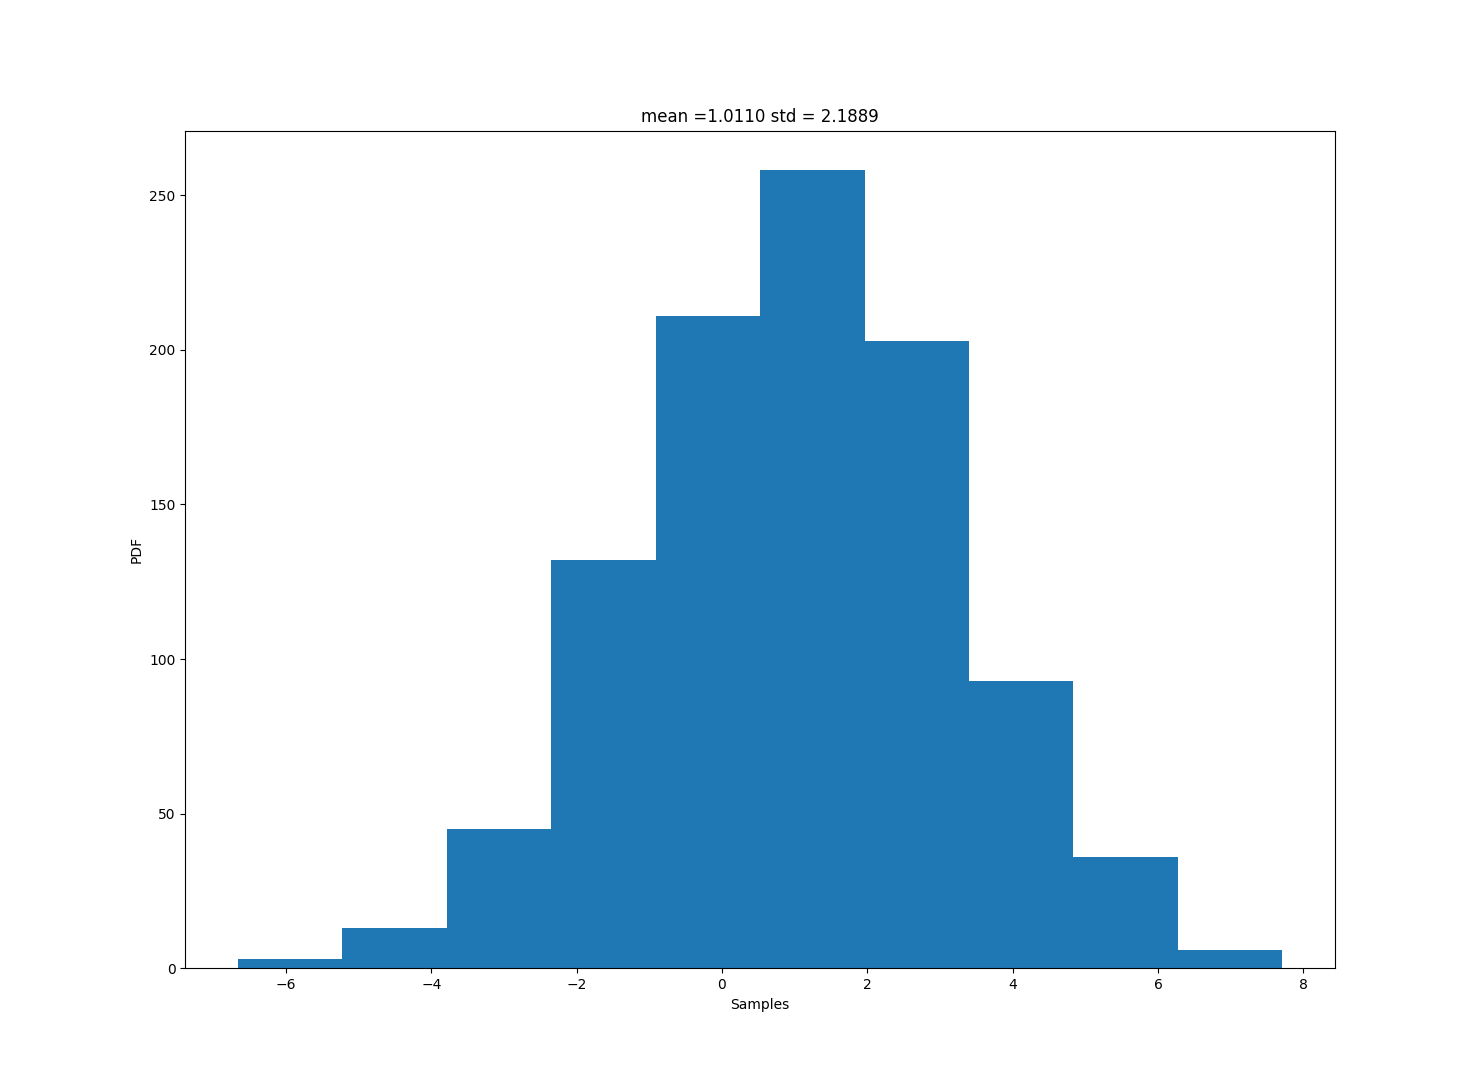
\includegraphics[width=\textwidth]{Eval/GaussianUnitTest.png}
		\captionof{figure}{Program 1: The Gaussian unit test with mean: 1 std: $\sqrt{5}$}
	\end{center}

	\begin{center}
		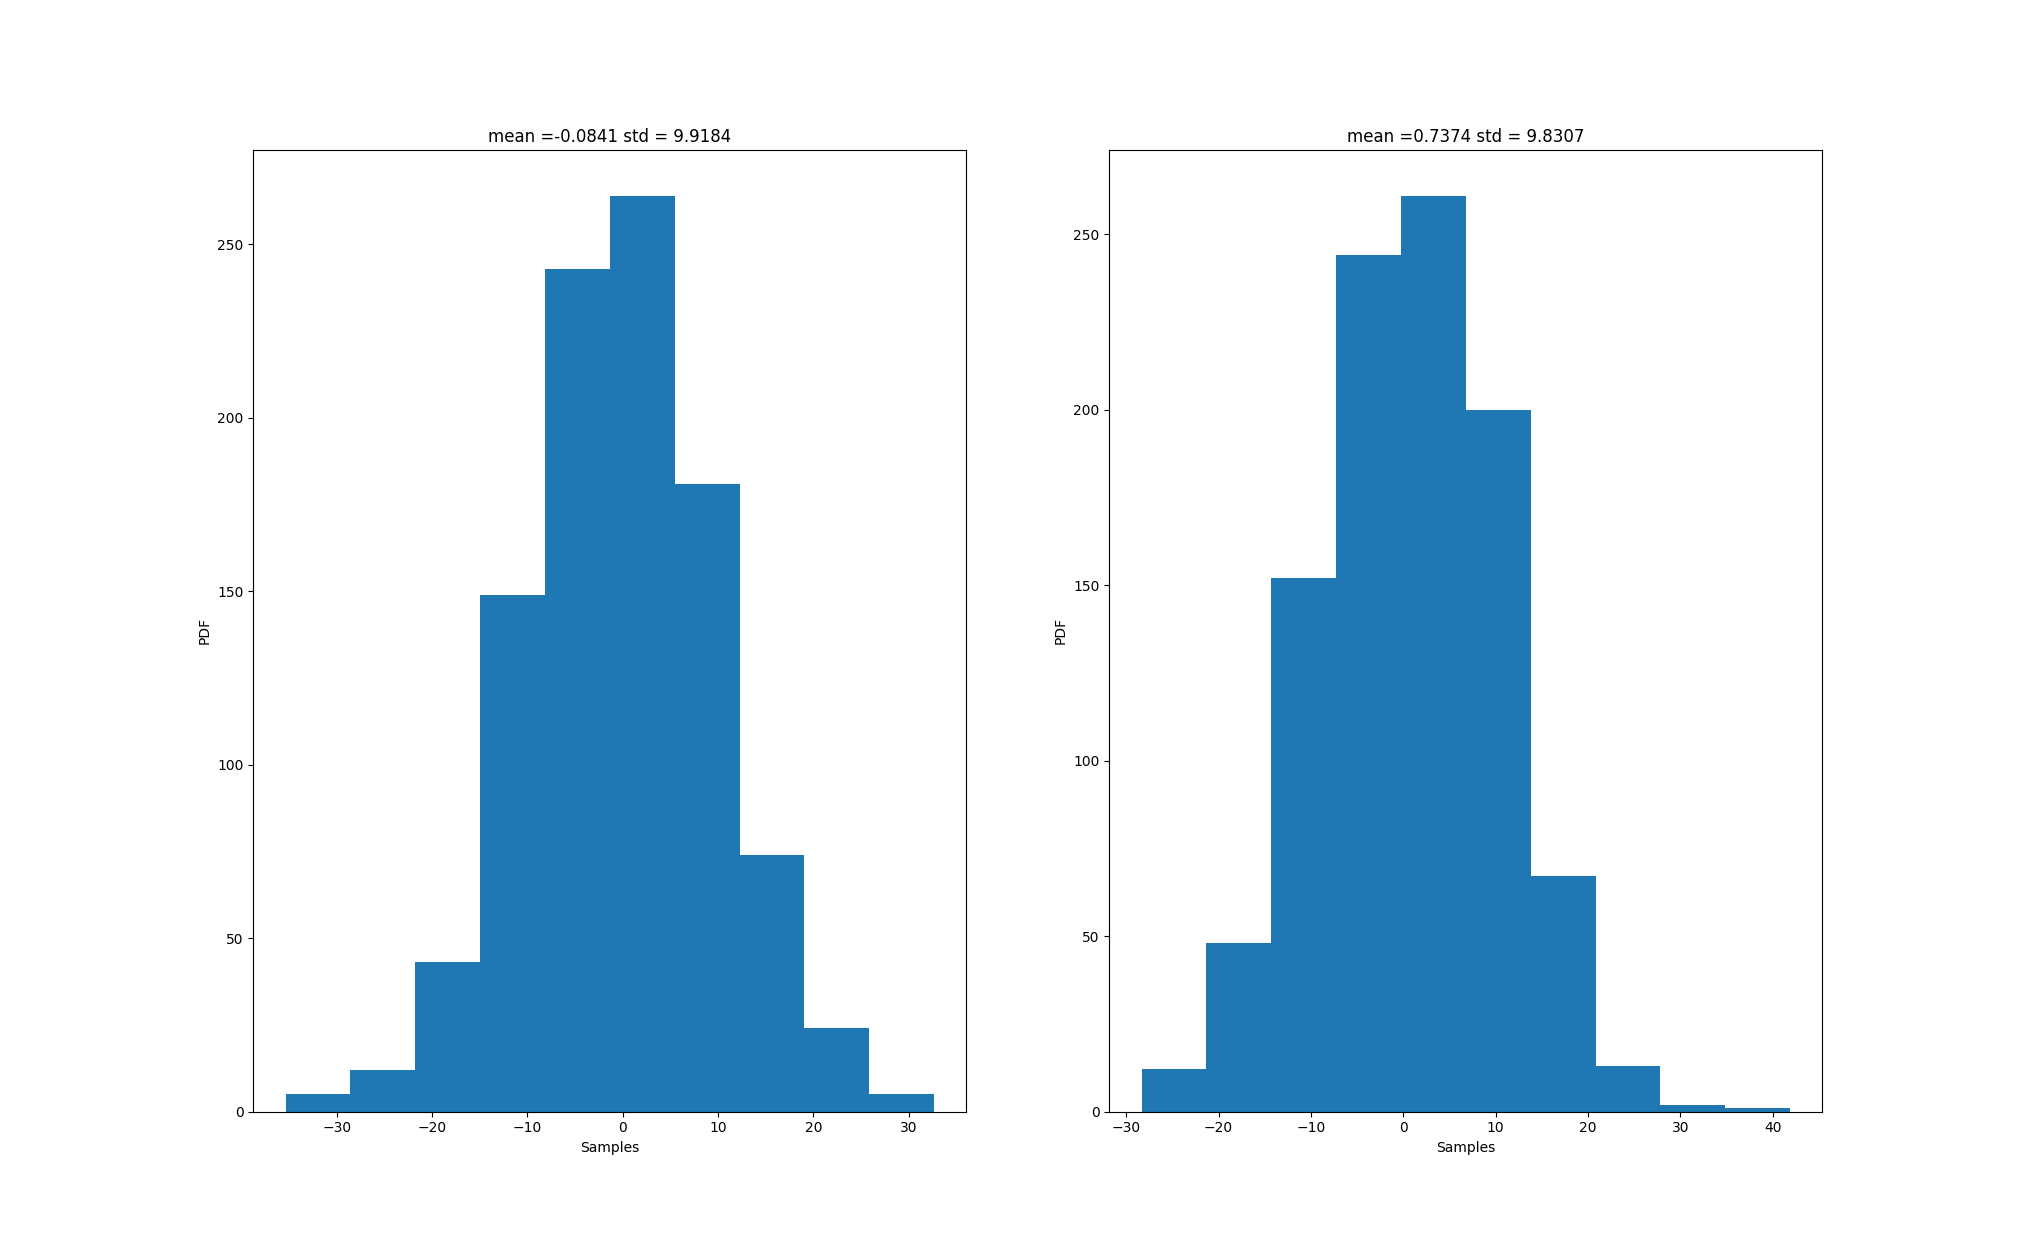
\includegraphics[width=\textwidth]{Eval/BayesianLinearReg.png}
		\captionof{figure}{Program 2: The Bayesian linear regression with slope and bias mean:0 std: 10. The plot on the left is the slope and the one on the right is the bias}
	\end{center}



	\begin{center}
		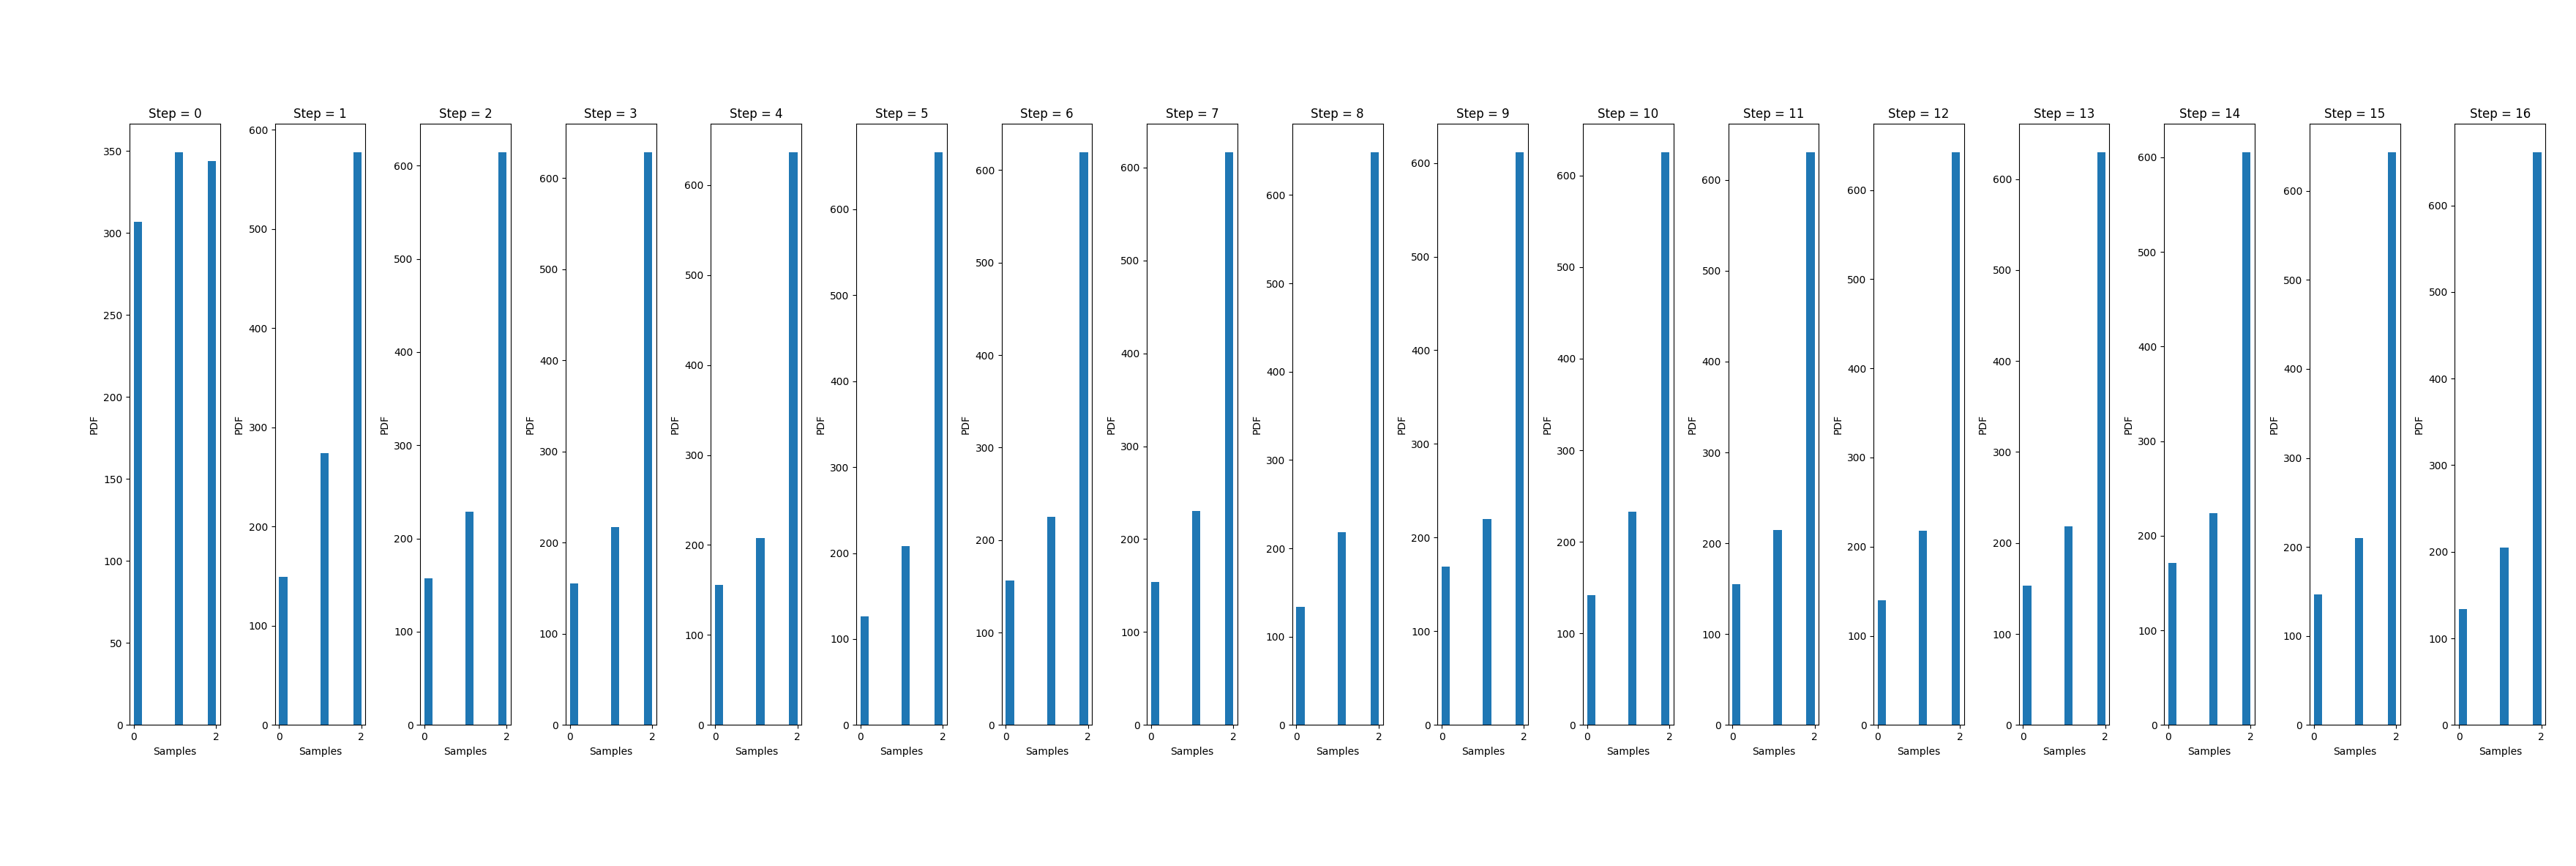
\includegraphics[width=\textwidth]{Eval/HMM.png}
		\captionof{figure}{Program 3: The HMM distribution of states is shown at each time step}
	\end{center}

The histograms from time step 3 onwards the distribution of states appears to have converged. In step 0 as denoted in the program the distribution of states is roughly equal.
\newpage
The Bayesian Neural Network returns the distribution for $W_0$, $b_0$, $W_1$ and $b_1$.

	\begin{center}
		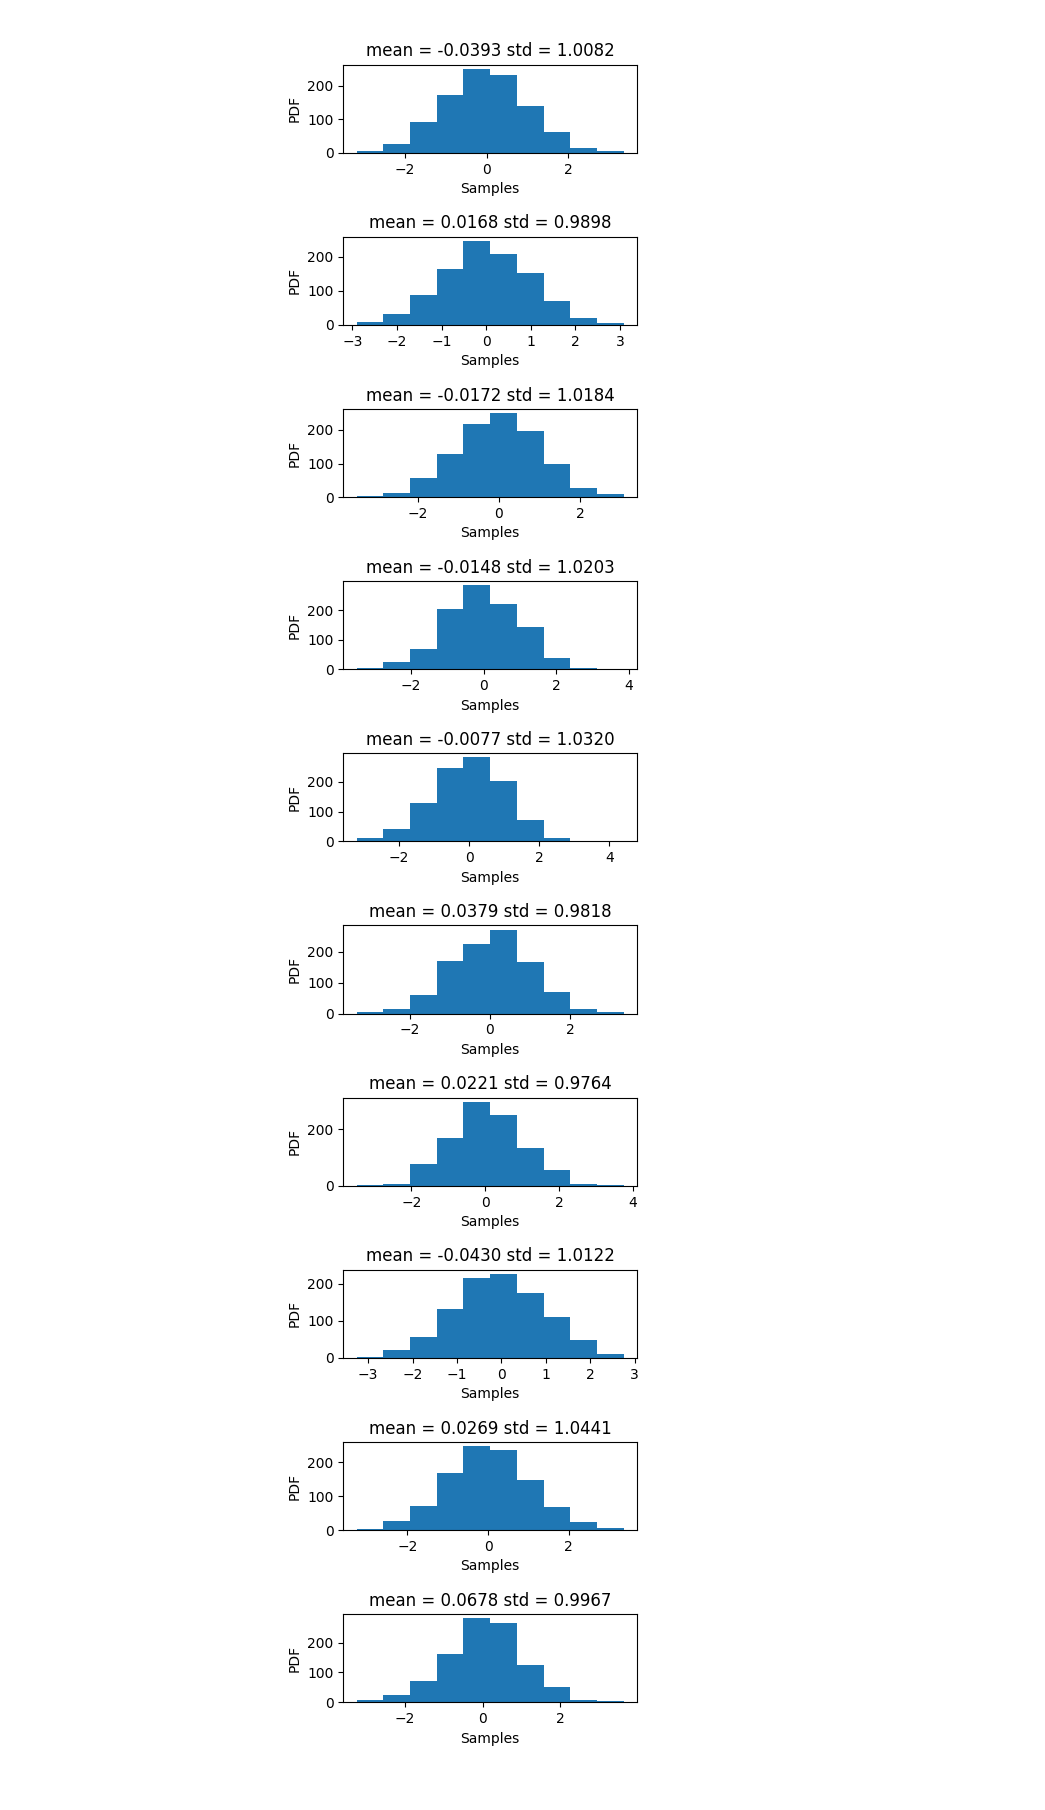
\includegraphics[height=.8\textheight]{Eval/W0_nn.png}
		\captionof{figure}{Program 4: The Bayesian Neural Network weights $W_0$ from top to bottom are the corresponding $i=0$ to $i=9$ histograms for the $10\times1$ vector of $W_0$ (zoom in to see mean and std)}
	\end{center}


	\begin{center}
		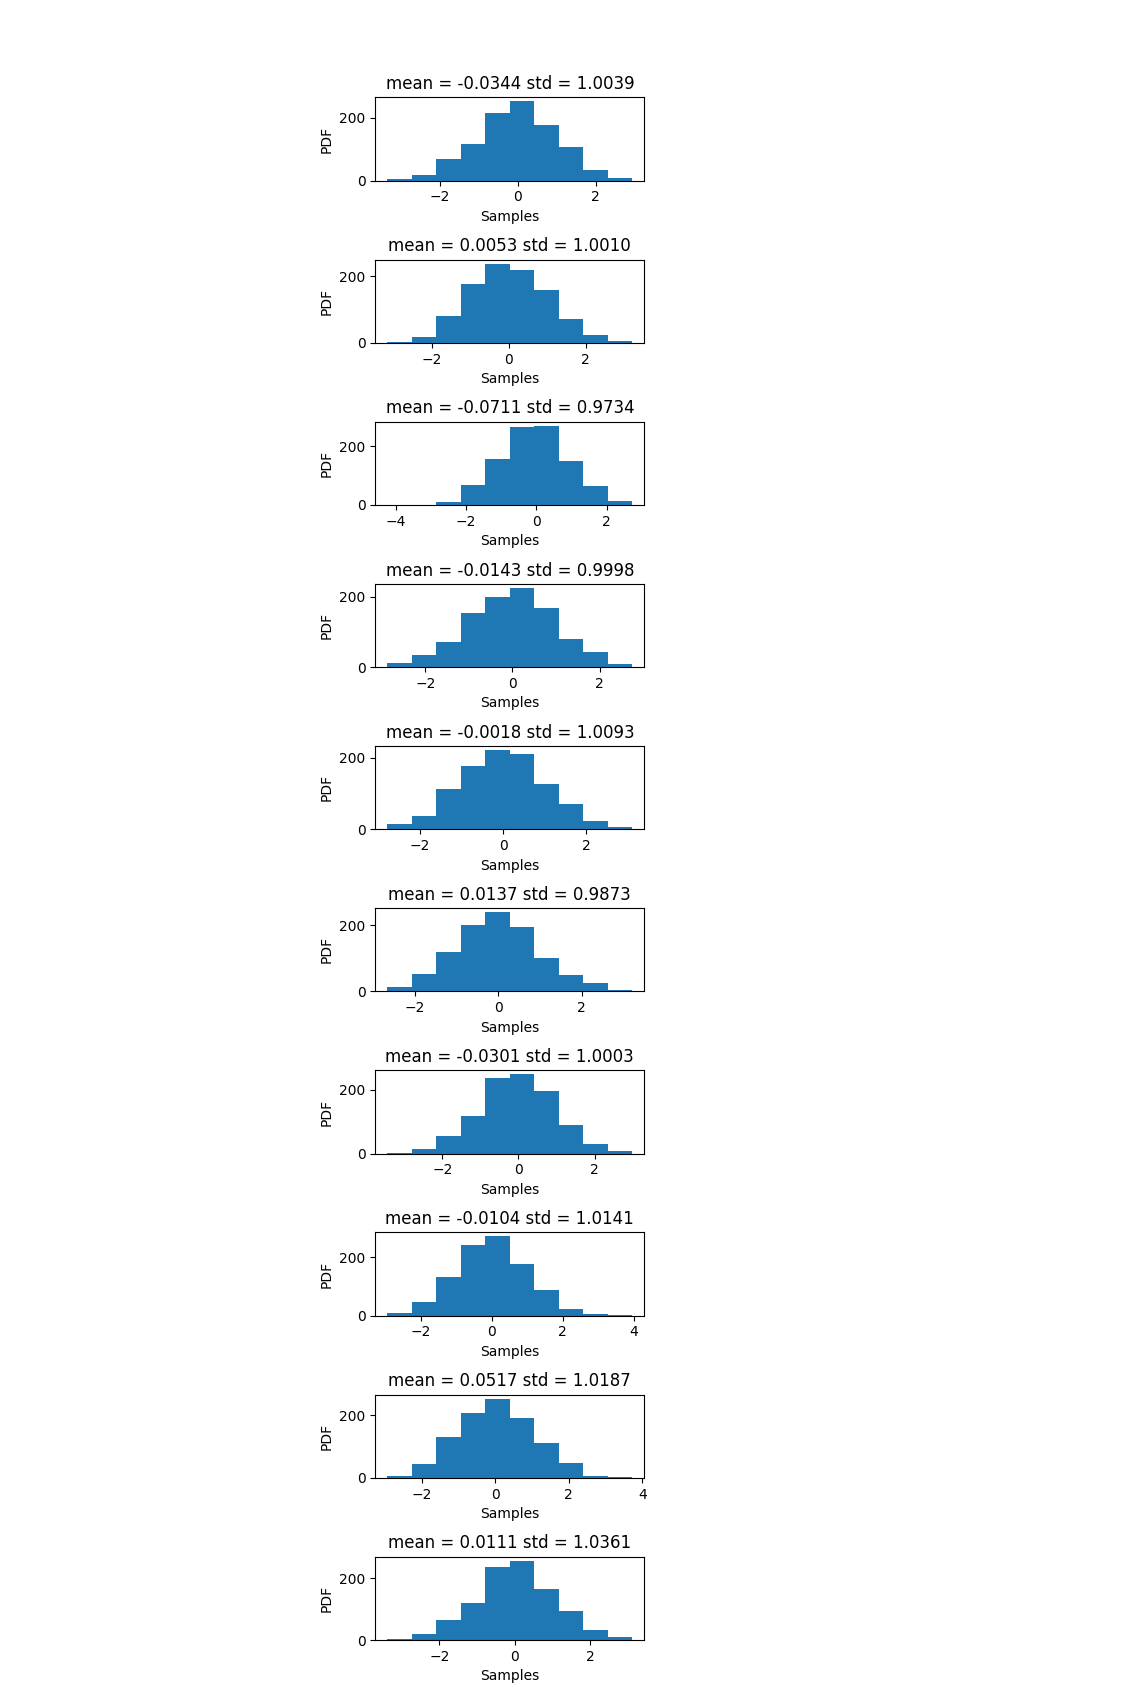
\includegraphics[height=.9\textheight]{Eval/b0_nn.png}
		\captionof{figure}{Program 4: The Bayesian Neural Network weights $b_0$ from top to bottom are the corresponding $i=0$ to $i=9$ histograms for the $10\times1$ vector of $b_0$ (zoom in to see mean and std)}
	\end{center}


	\begin{center}
		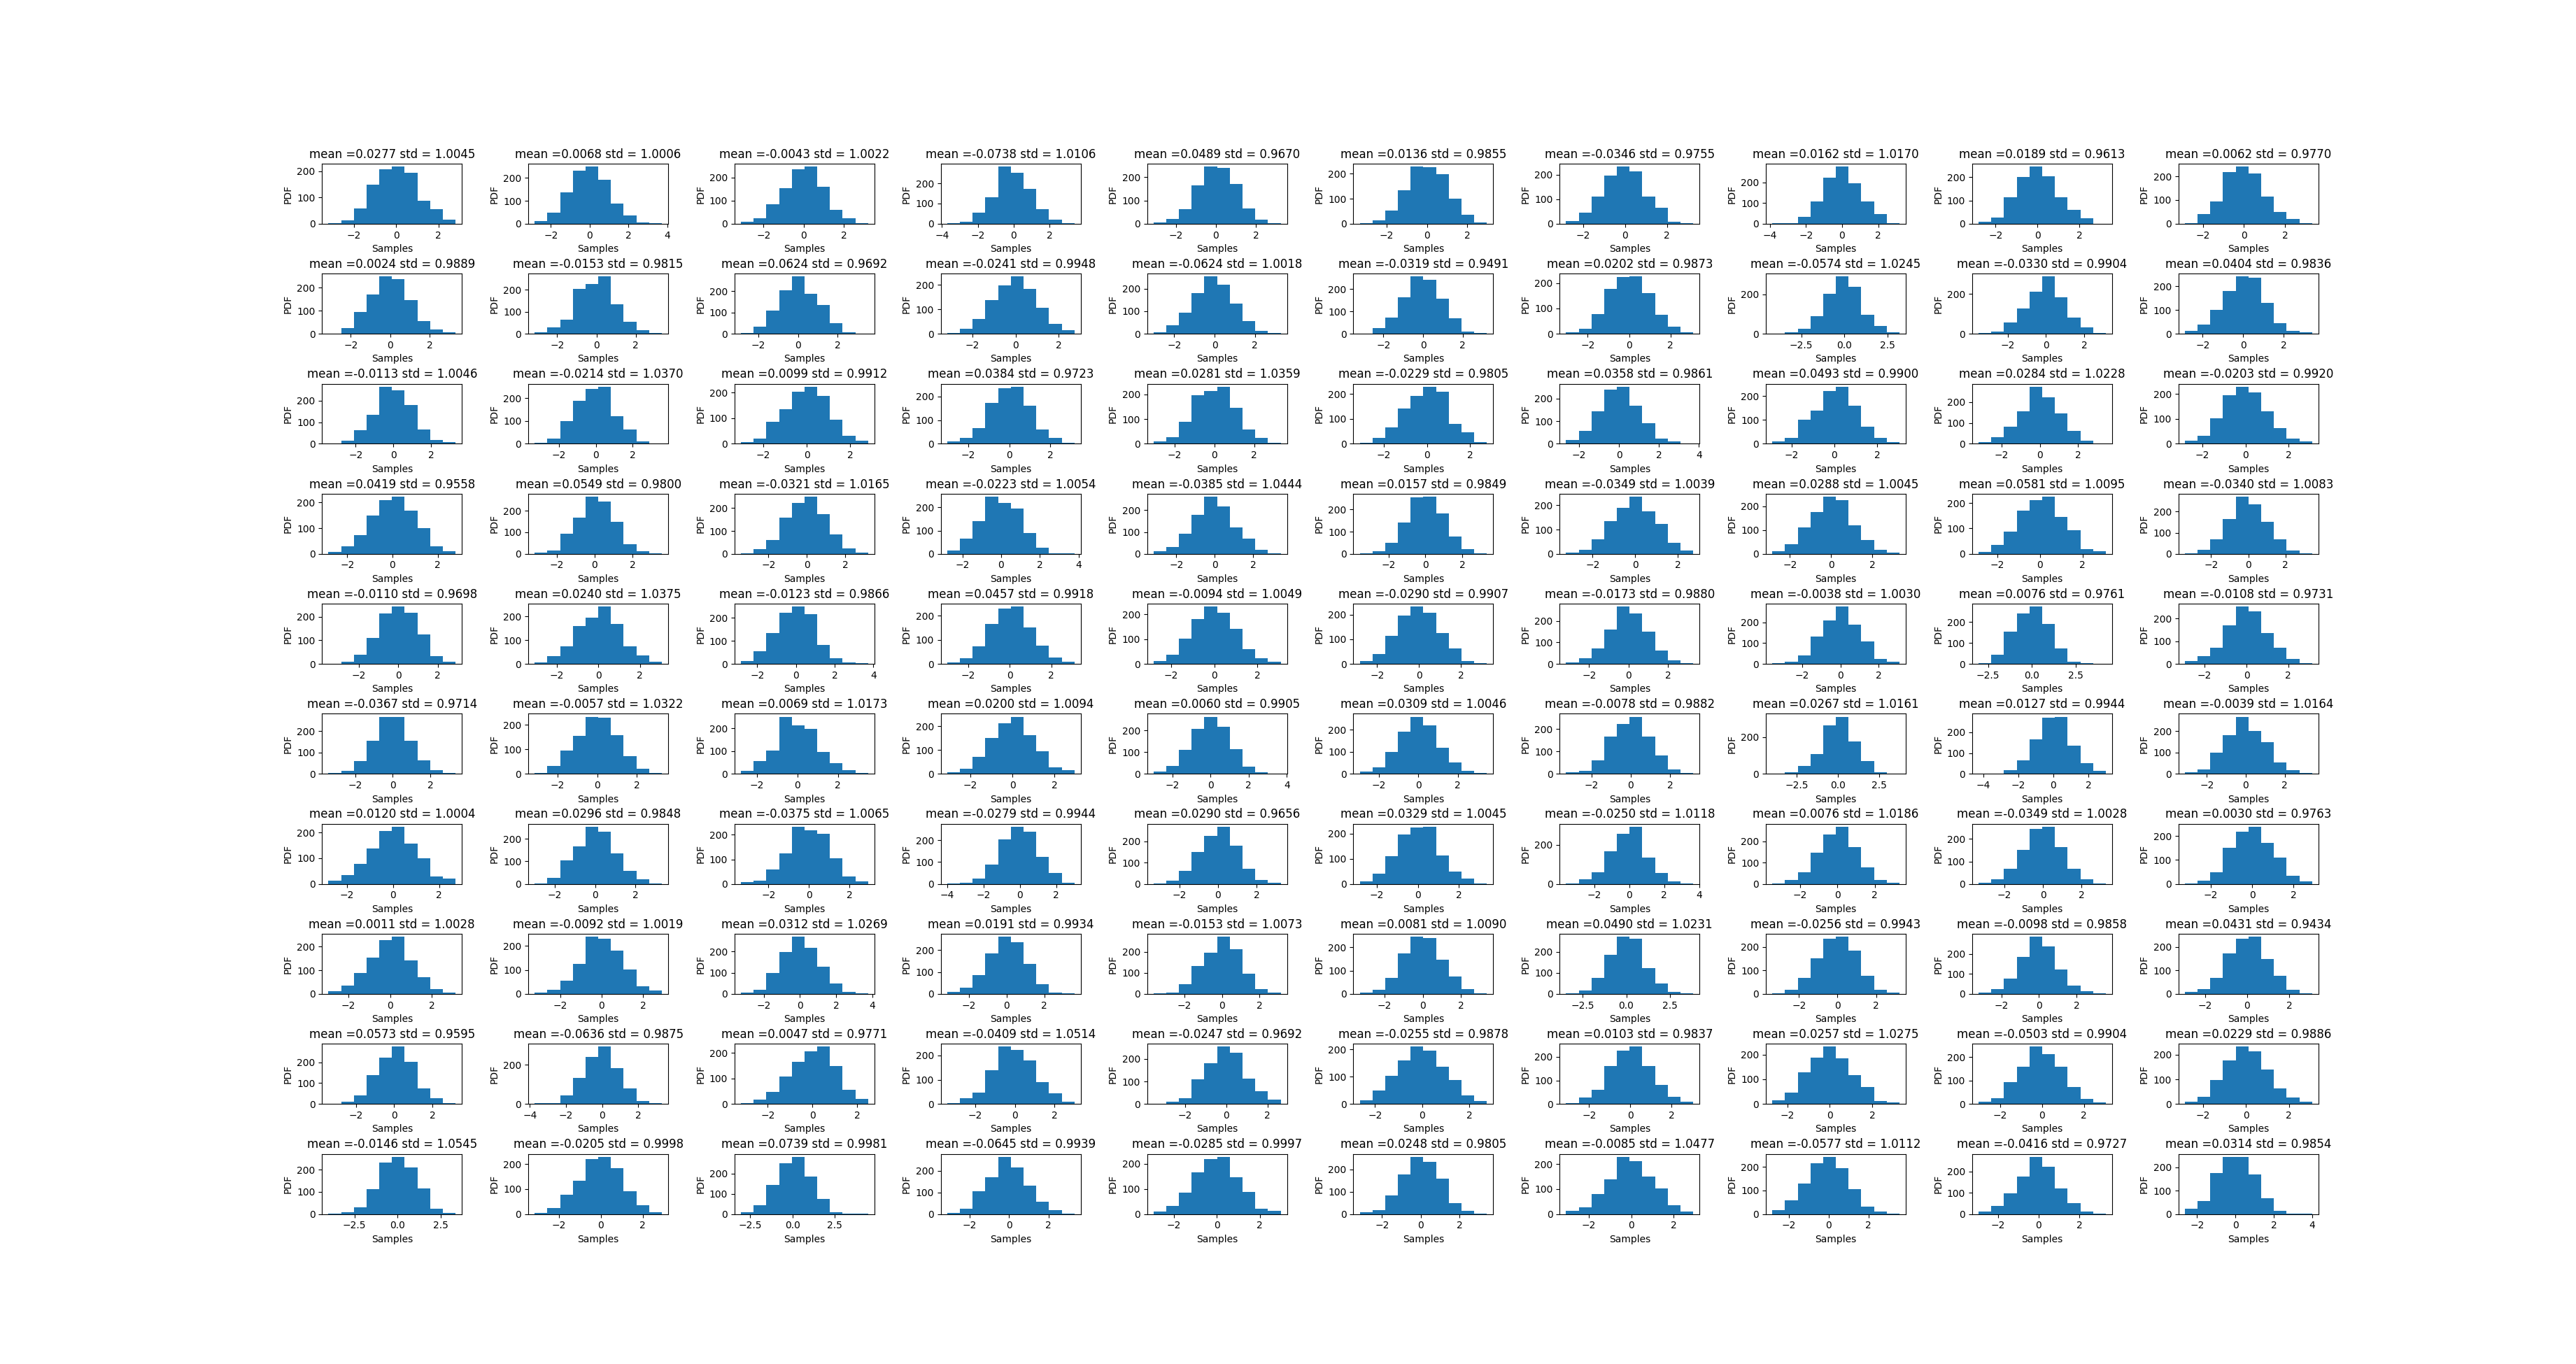
\includegraphics[width=\textwidth]{Eval/W1_nn.png}
		\captionof{figure}{Program 4: The Bayesian Neural Network weights $W_1$. The histograms are oriented in the same configuration as the $W_1$ matrix i.e histogram $i,j$ corresponds to element $i,j$ of $W_1$ where $W_1$ is a $10\times10$ matrix. Here $i$ corresponds to rows, $j$ to columns.(Zoom in to see the mean and std)}
	\end{center}


	\begin{center}
		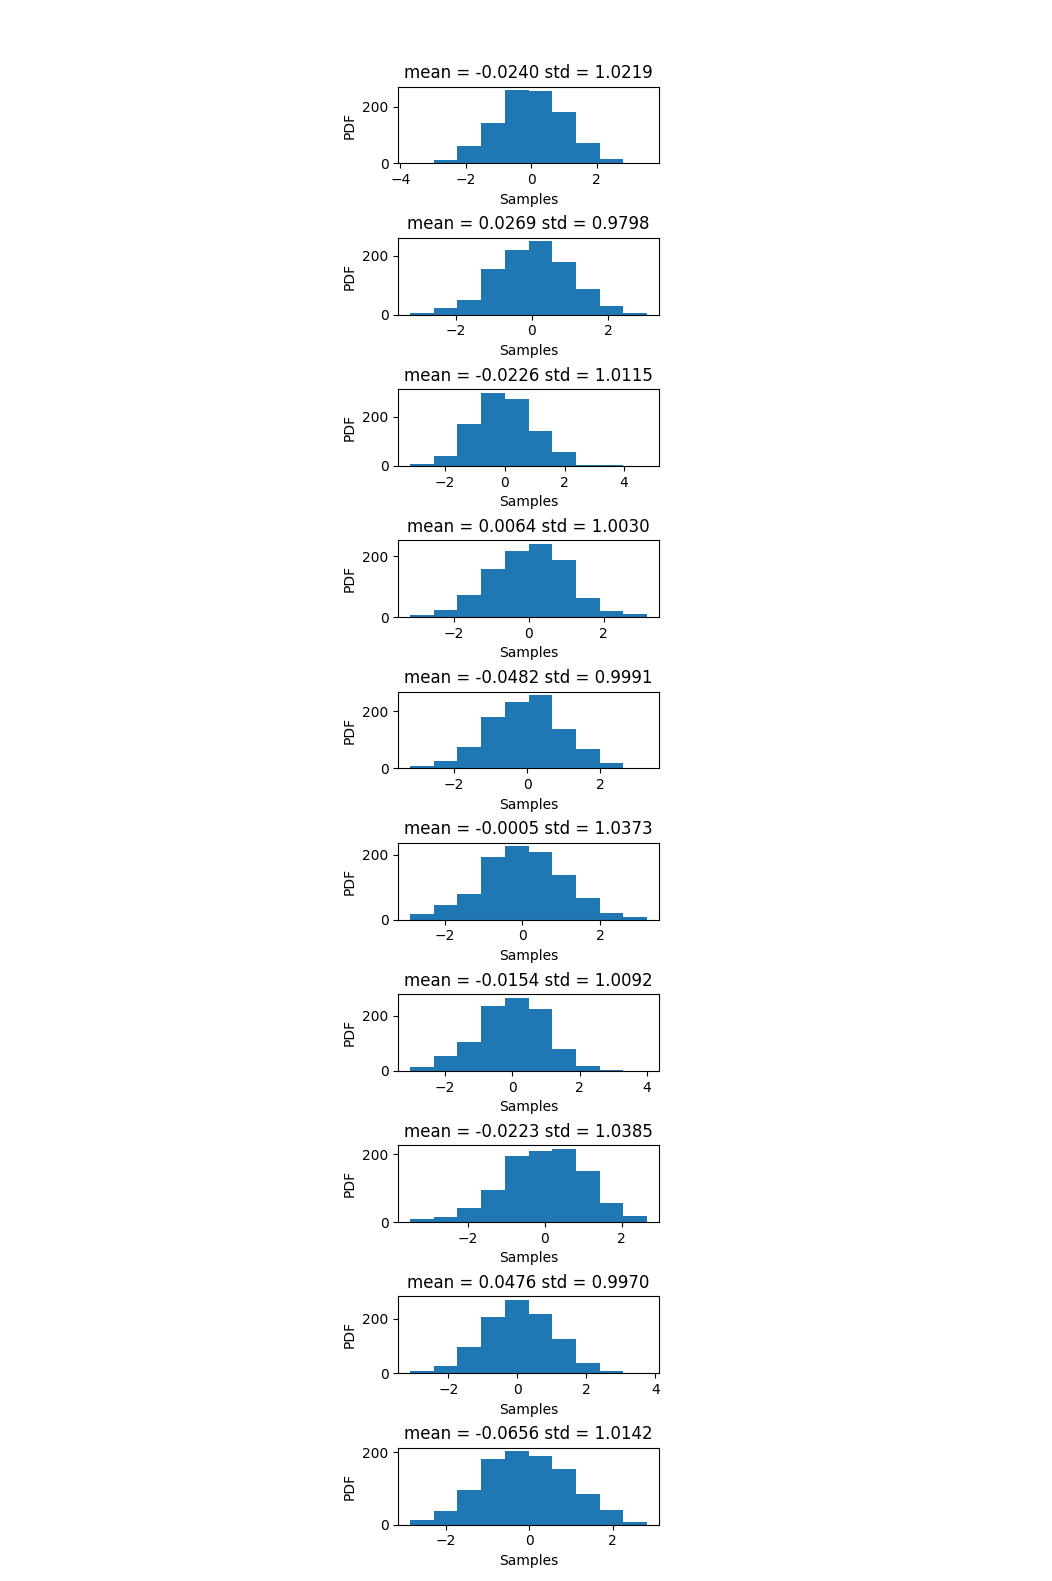
\includegraphics[height=.8\textheight]{Eval/b1_nn.png}
		\captionof{figure}{Program 4: The Bayesian Neural Network weights $b_1$ from top to bottom are the corresponding $i=0$ to $i=9$ histograms for the $10\times1$ vector of $b_1$ (zoom in to see mean and std)}
	\end{center}



\section{Graph Based Sampling}
The strategy in graph based sampling is a non-standard execution to achieve the same meaning as the evaluation based sampling. Similar to the previous part, Pytorch and tensors are used. The primitive functions implemented is the same:

\lstinputlisting[language = Python,linerange = {13-40} ]{graph_based_sampling.py}

The deterministic function evaluations makes calls to the primitive functions in:
\lstinputlisting[language = Python,linerange = {6-6} ]{graph_based_sampling.py}
The deterministic evaluation is as follows:
\lstinputlisting[language = Python,linerange = {43-54} ]{graph_based_sampling.py}

And the \emph{funcprimitives} are defined as:
\lstinputlisting[language = Python,linerange = {3-33} ]{primitives.py}

In order to construct the vectors and matrices properly, \emph{torch.stack} is used to appropriately construct list of lists which allows us to define vectors and matrices. Similarly to the evaluation based sampling, \emph{sample} and \emph{observe} are treated the same. The control flow \emph{if} is evaluated lazily here, but I acknowledge that when observes come into play this will need to be modified.

In order to do ancestral sampling, a topological sort of the vertices needs to be performed. I implemented Kahn's algorithm from:
\begin{center}
	\url{https://www.geeksforgeeks.org/topological-sorting-indegree-based-solution/} 
\end{center} 
Note a more concise implementation likely exists:
\lstinputlisting[language = Python,linerange = {45-92} ]{primitives.py}
Of note, if the sorting cannot be performed, then I return the list of vertices.
Once the vertices are sorted, then I bind vertex nodes with their samples from the link functions in $P$ by binding variables to values in \emph{bindingVars} which recursively unpacks lists and binds variables to values:
 \lstinputlisting[language = Python,linerange = {35-42} ]{primitives.py}

Thus to perform ancestral sampling the steps are extract vertices $V$ and edges $A$ from the graph. Topological sort $V$, get the link functions from $P$ and execute the link function from $P$ and store the results in a dictionary $R$. Sample each $V$ in the sorted order making calls to $P$. Once each node $V$ has a value, then the \emph{bindingVars} function is called to return the expression of the program stored in $E$. \emph{sample\_from\_joint} is shown:
  \lstinputlisting[language = Python,linerange = {57-82} ]{primitives.py}
\newpage
\subsection{Results}
Similar to the evaluation based sampling, the results are summarized here:.
\begin{verbatim}
Test passed
Test passed
Test passed
Test passed
Test passed
Test passed
Test passed
Test passed
Test passed
Test passed
Test passed
Test passed
All deterministic tests passed
('normal', 5, 1.4142136)
p value 0.7468519478136475
('beta', 2.0, 5.0)
p value 0.9760889086114111
('exponential', 0.0, 5.0)
p value 0.7425461404031451
('normal', 5.3, 3.2)
p value 0.319890341320916
('normalmix', 0.1, -1, 0.3, 0.9, 1, 0.3)
p value 0.3386100157743366
('normal', 0, 1.44)
p value 0.35515239218733097
All probabilistic tests passed
\end{verbatim}
\newpage
\begin{figure}[h]
	\begin{center}
		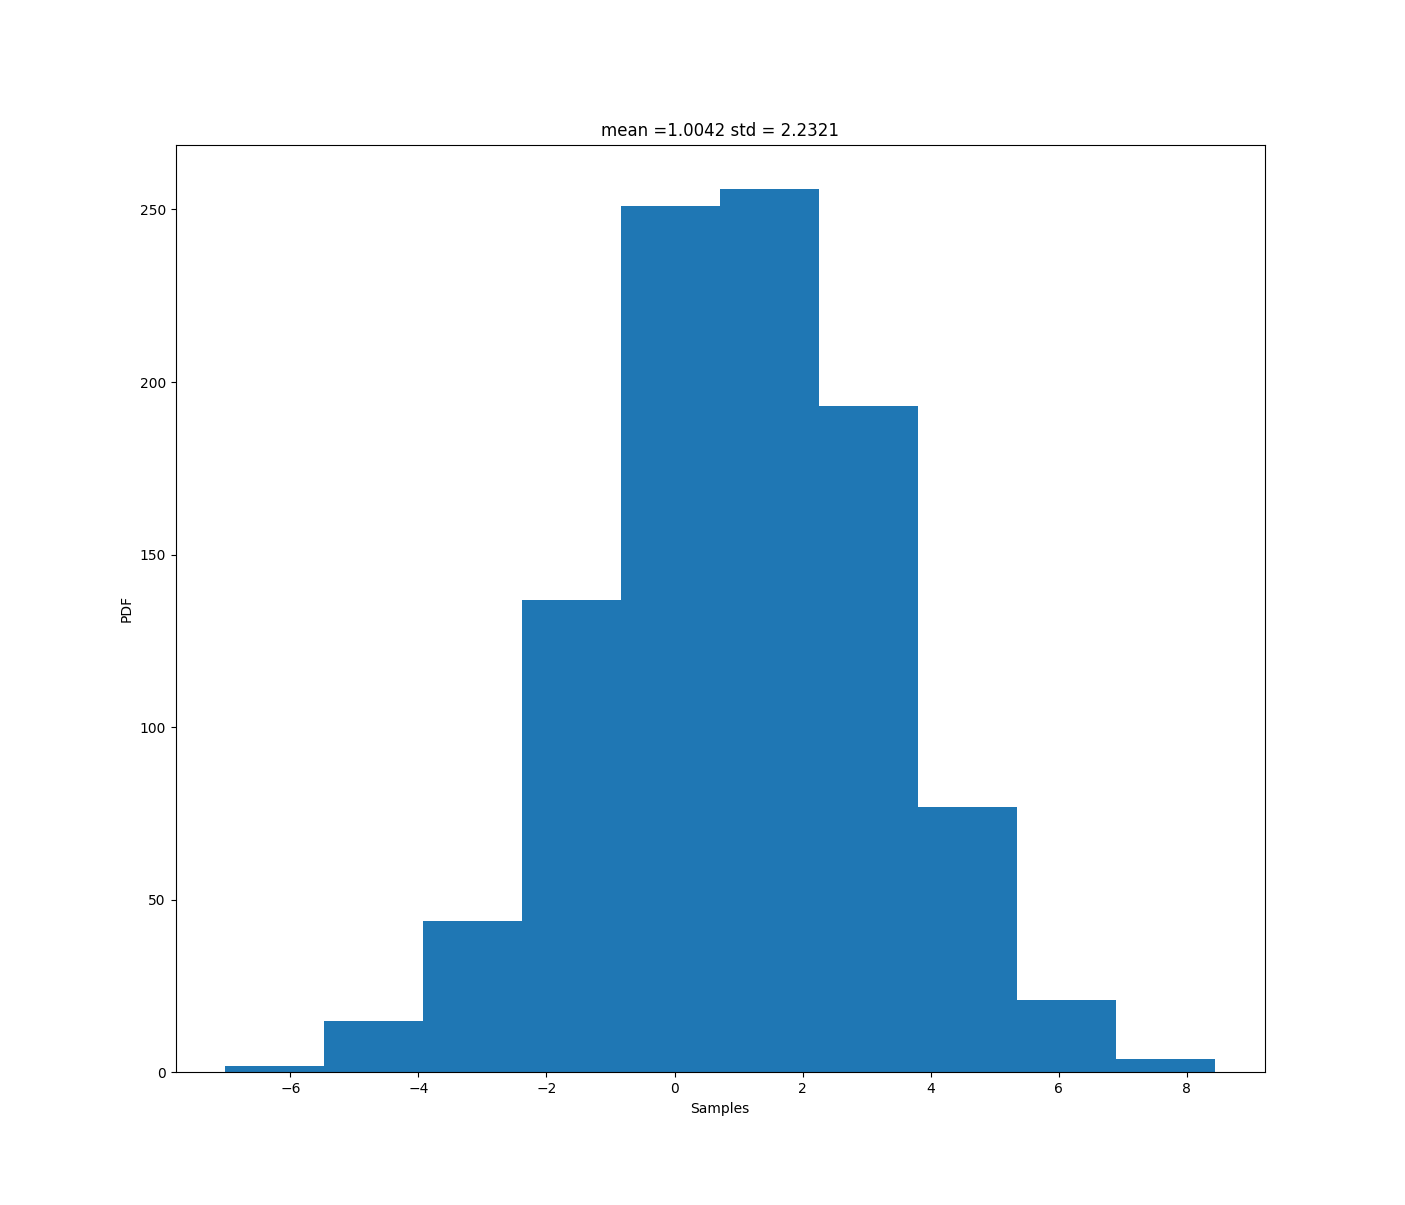
\includegraphics[width=\textwidth]{Graph/GaussianUnitTest.png}
		\caption{Program 1: The Gaussian unit test with mean: 1 std: $\sqrt{5}$}
	\end{center}
\end{figure}
\begin{figure}[h]
	\begin{center}
		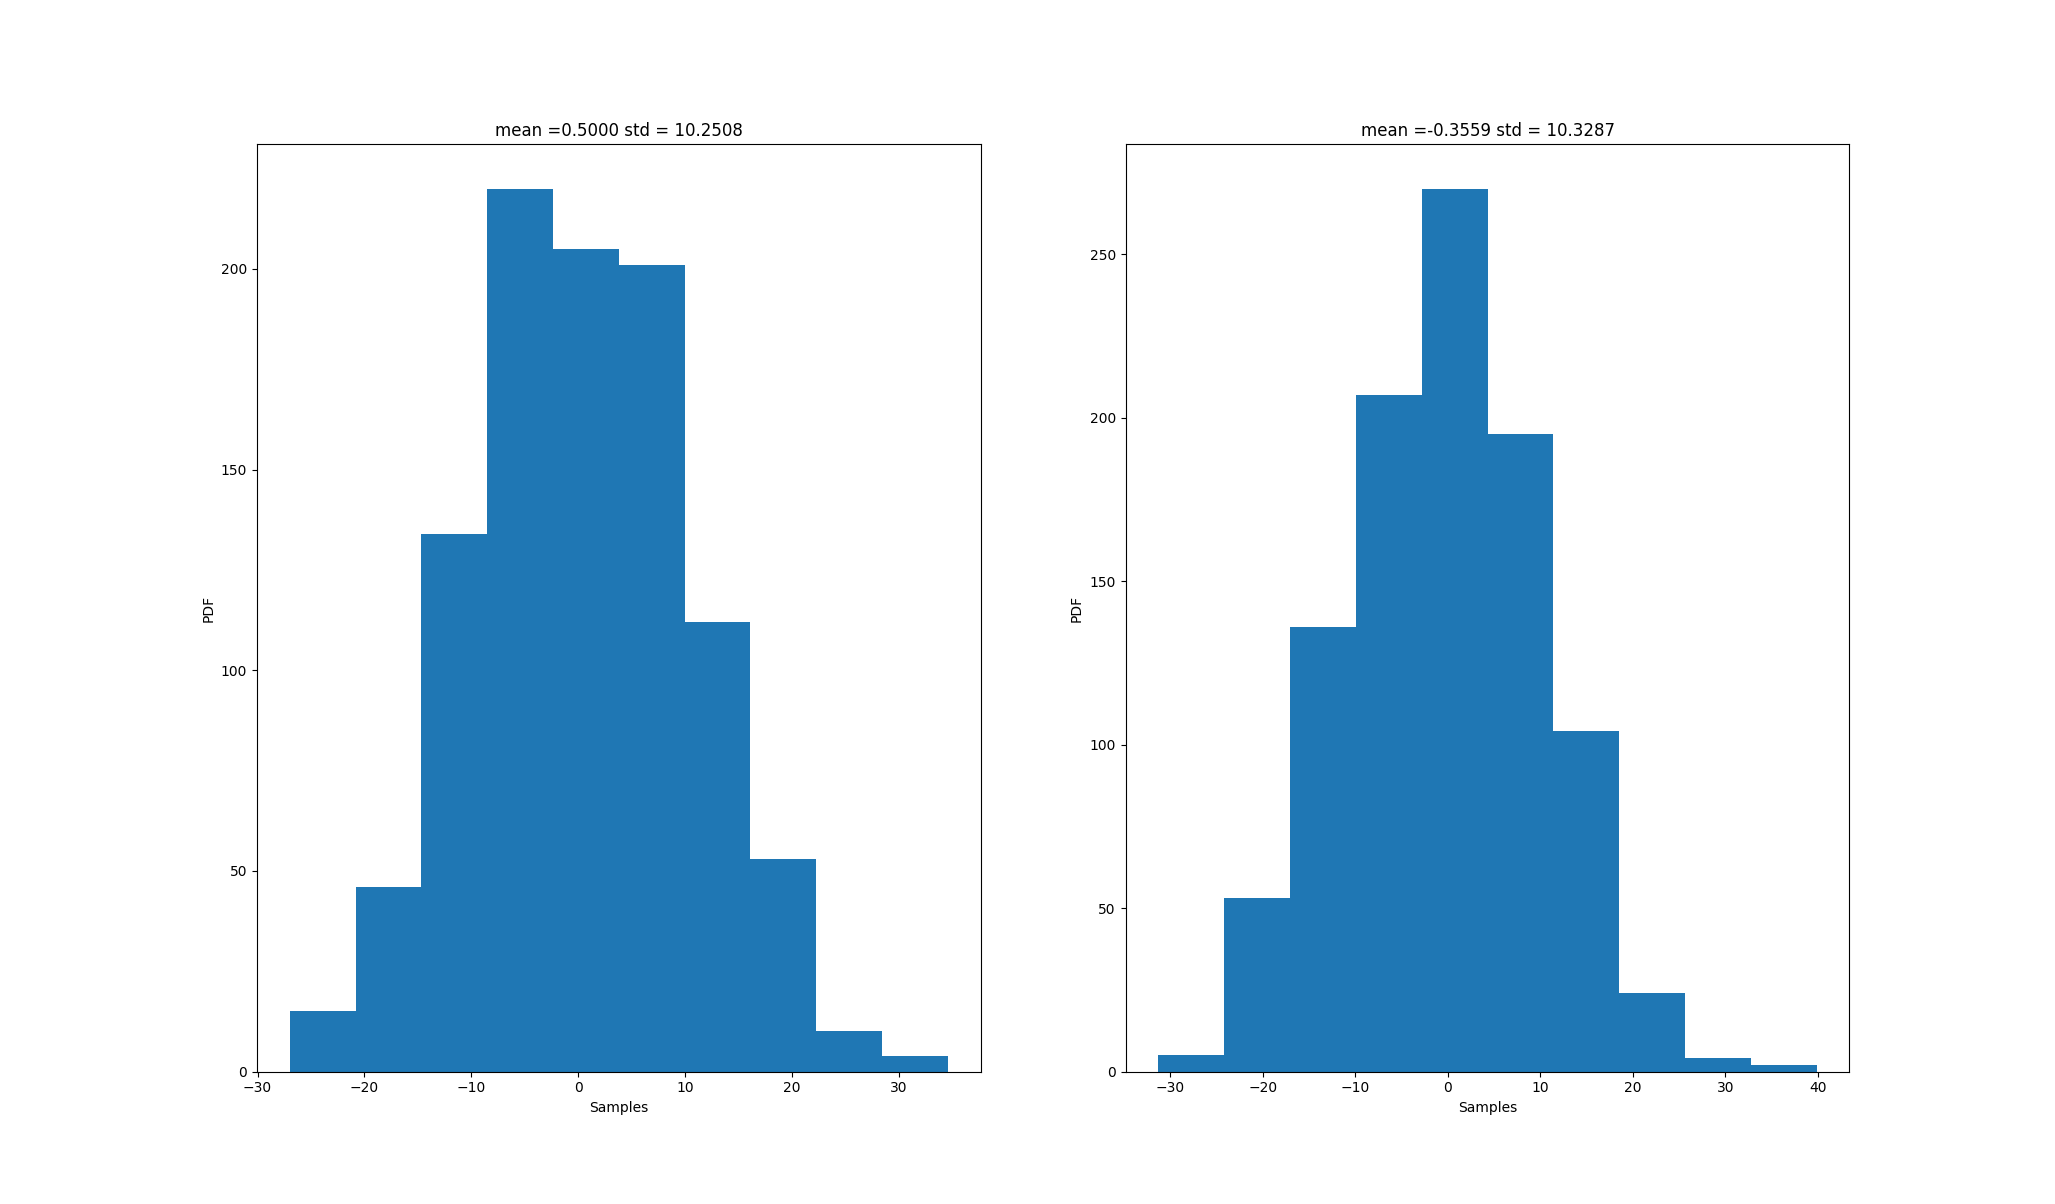
\includegraphics[width=\textwidth]{Graph/BayesianLinearReg.png}
		\caption{Program 2: The Bayesian linear regression with slope and bias mean:0 std: 10. The plot on the left is the slope and the one on the right is the bias}
	\end{center}
\end{figure}
\begin{figure}[h]
	\begin{center}
		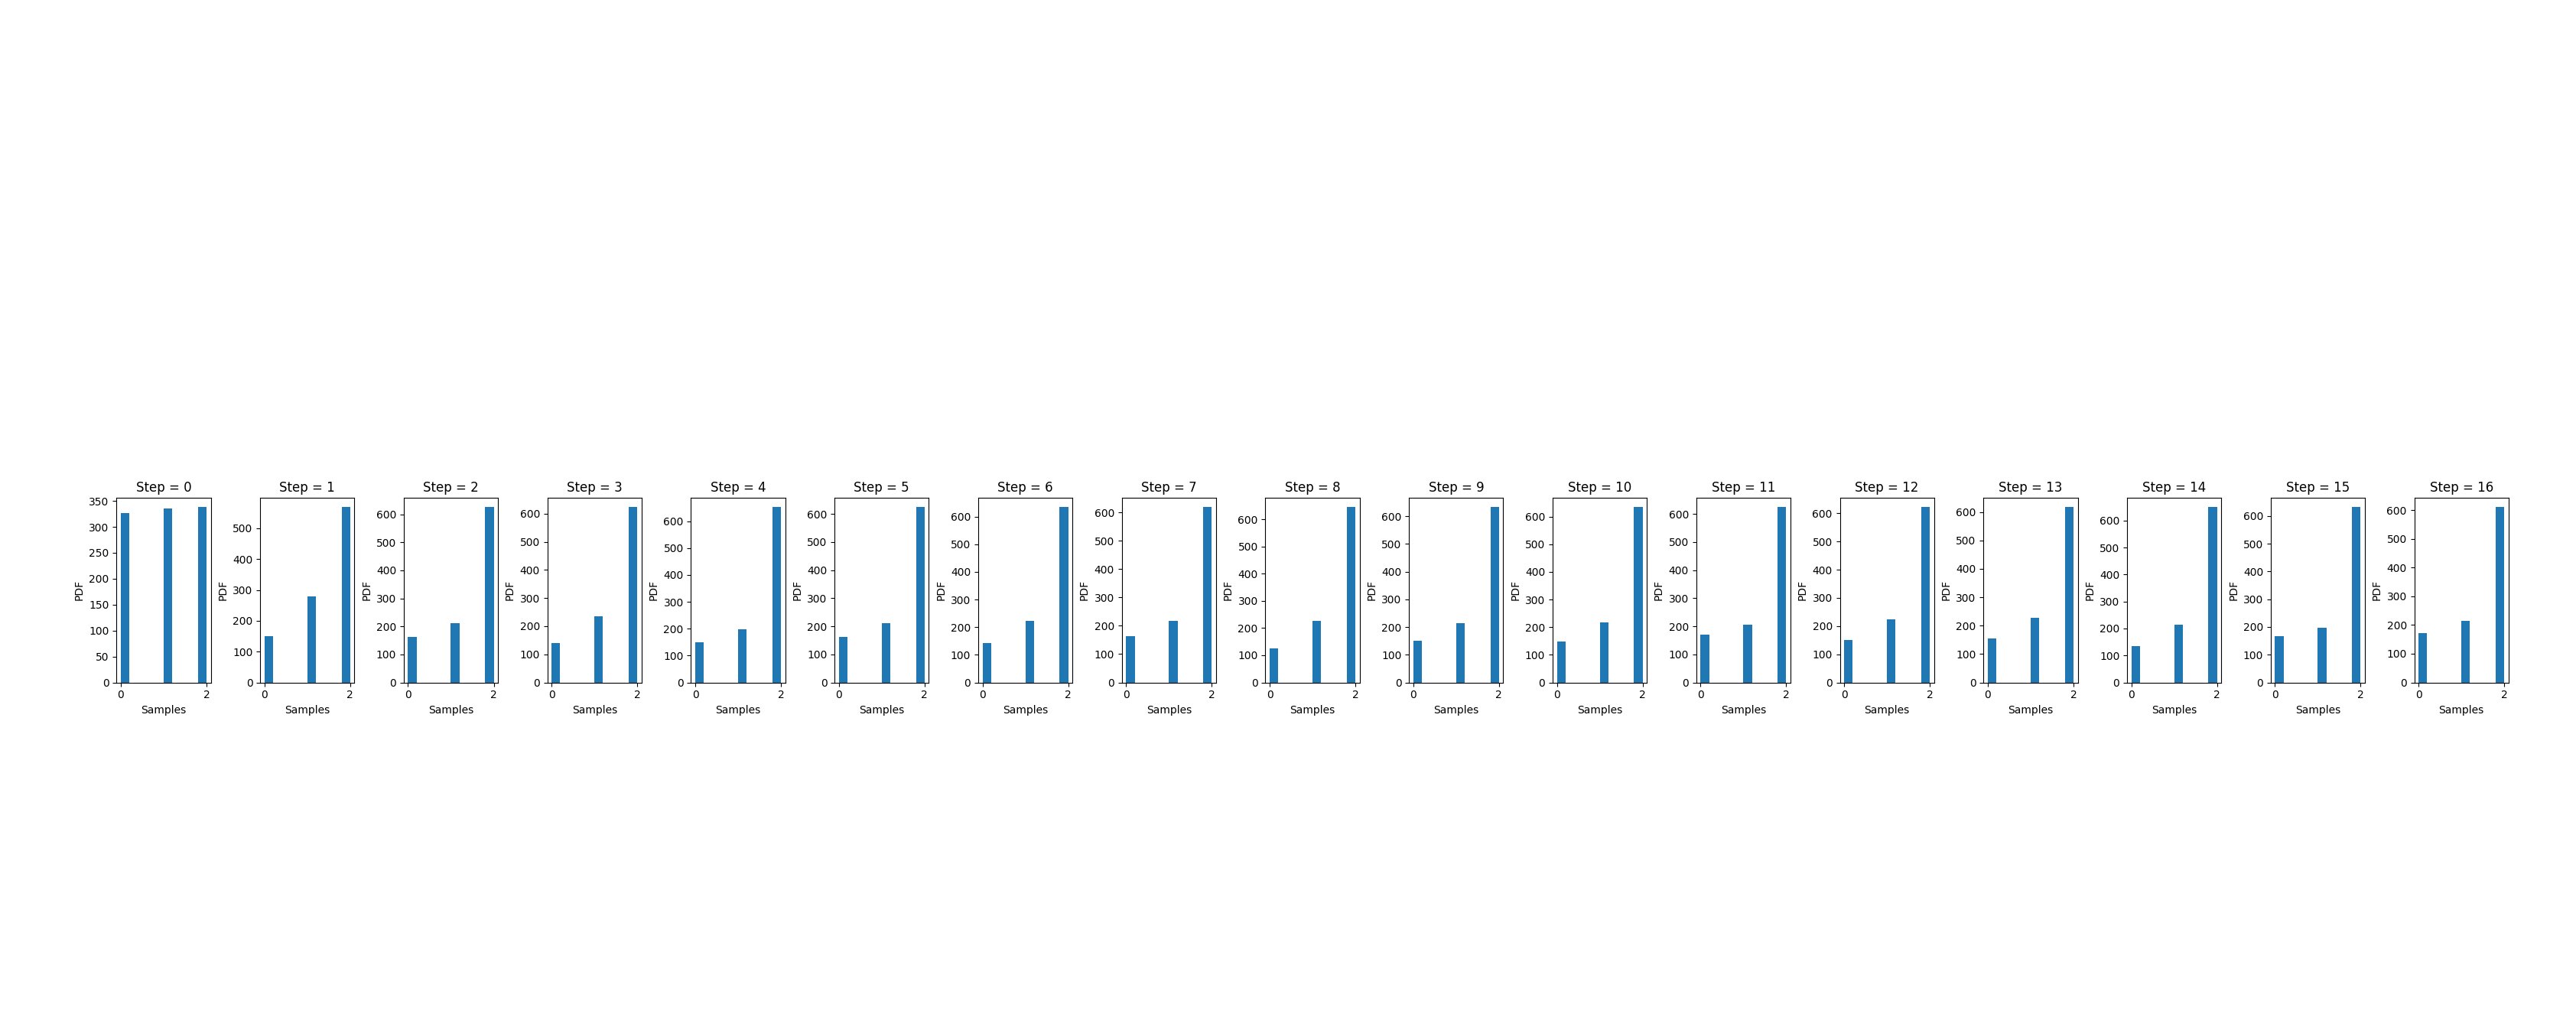
\includegraphics[width=\textwidth]{Graph/HMM.png}
		\caption{Program 3: The HMM distribution of states is shown at each time step}
	\end{center}
\end{figure}
The histograms from the evaluation based and graph based sampling produce similar results, i.e. after time step 3 the distribution of states appears to have converged. In step 0 as denoted in the program the distribution of states is roughly equal.

The Bayesian Neural Network returns the distribution for $W_0$, $b_0$, $W_1$ and $b_1$.
\begin{figure}[h]
	\begin{center}
		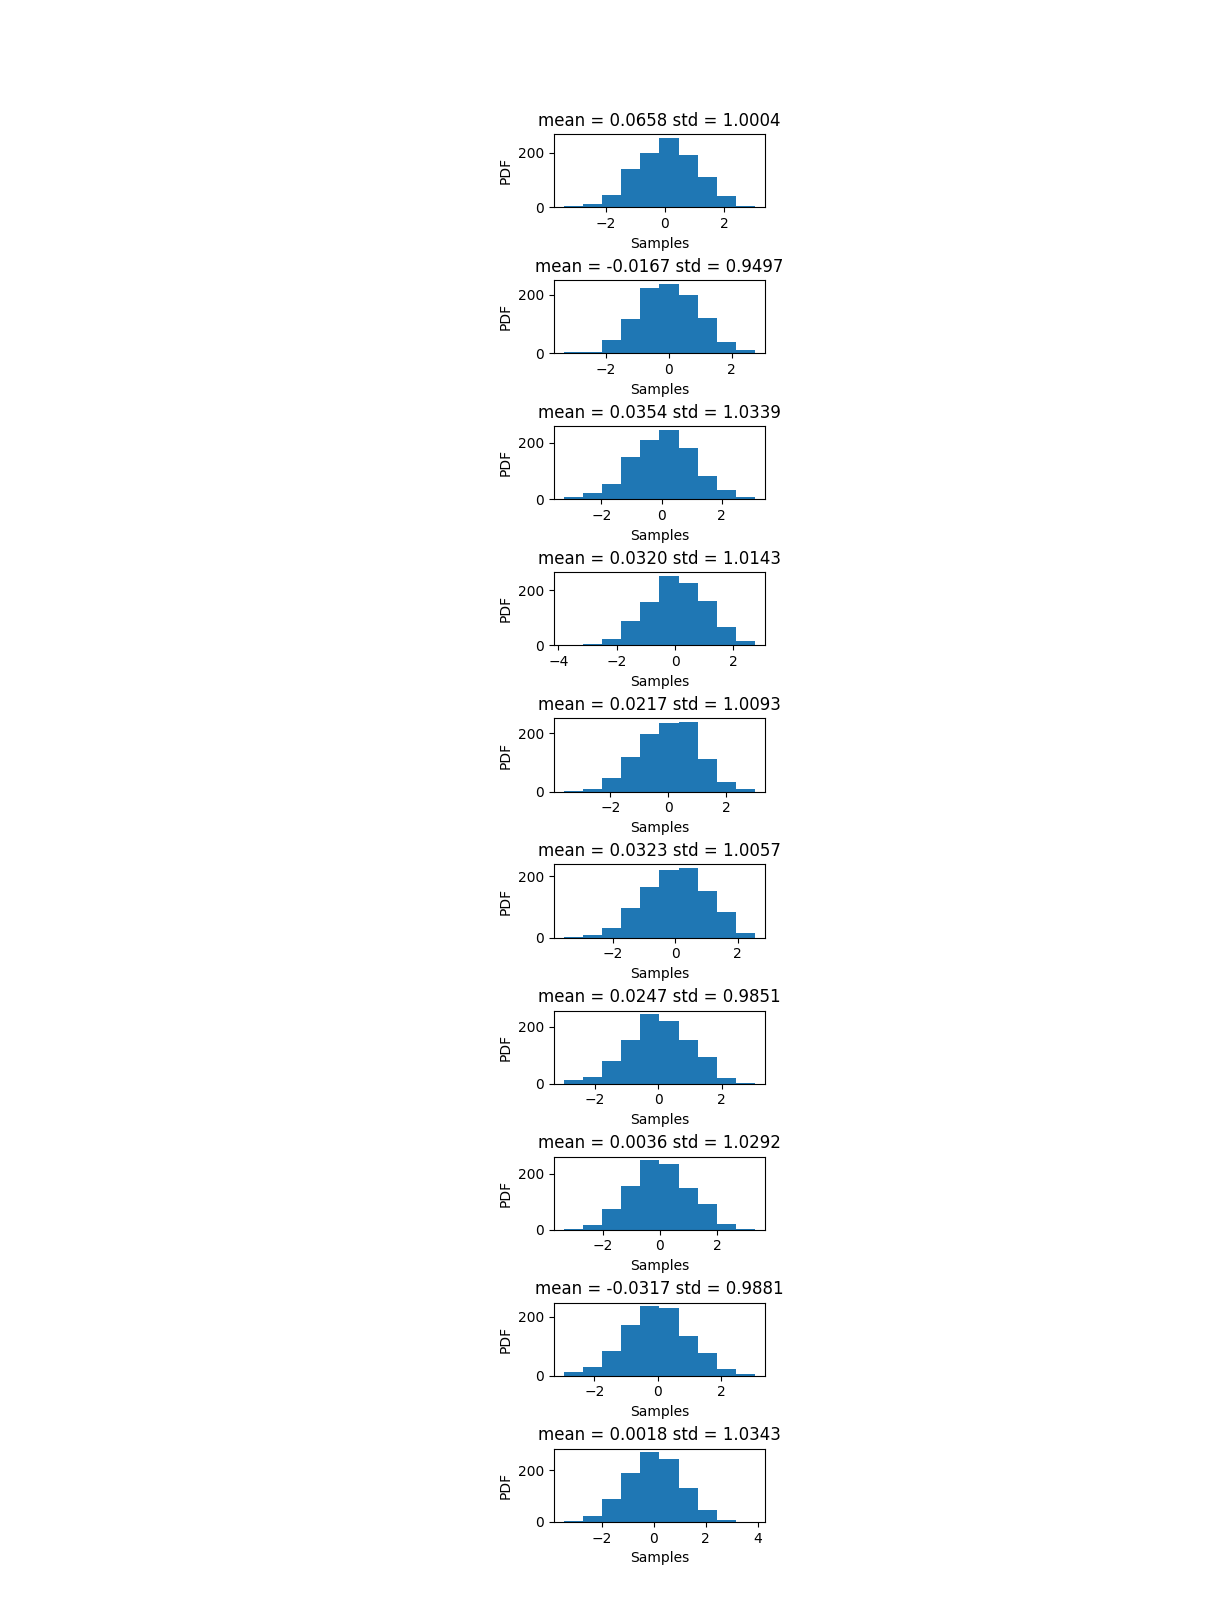
\includegraphics[width=\textwidth]{Graph/W0_nn.png}
		\caption{Program 4: The Bayesian Neural Network weights $W_0$ from top to bottom are the corresponding $i=0$ to $i=9$ histograms for the $10\times1$ vector of $W_0$ (zoom in to see mean and std)}
	\end{center}
\end{figure}
\begin{figure}[h]
	\begin{center}
		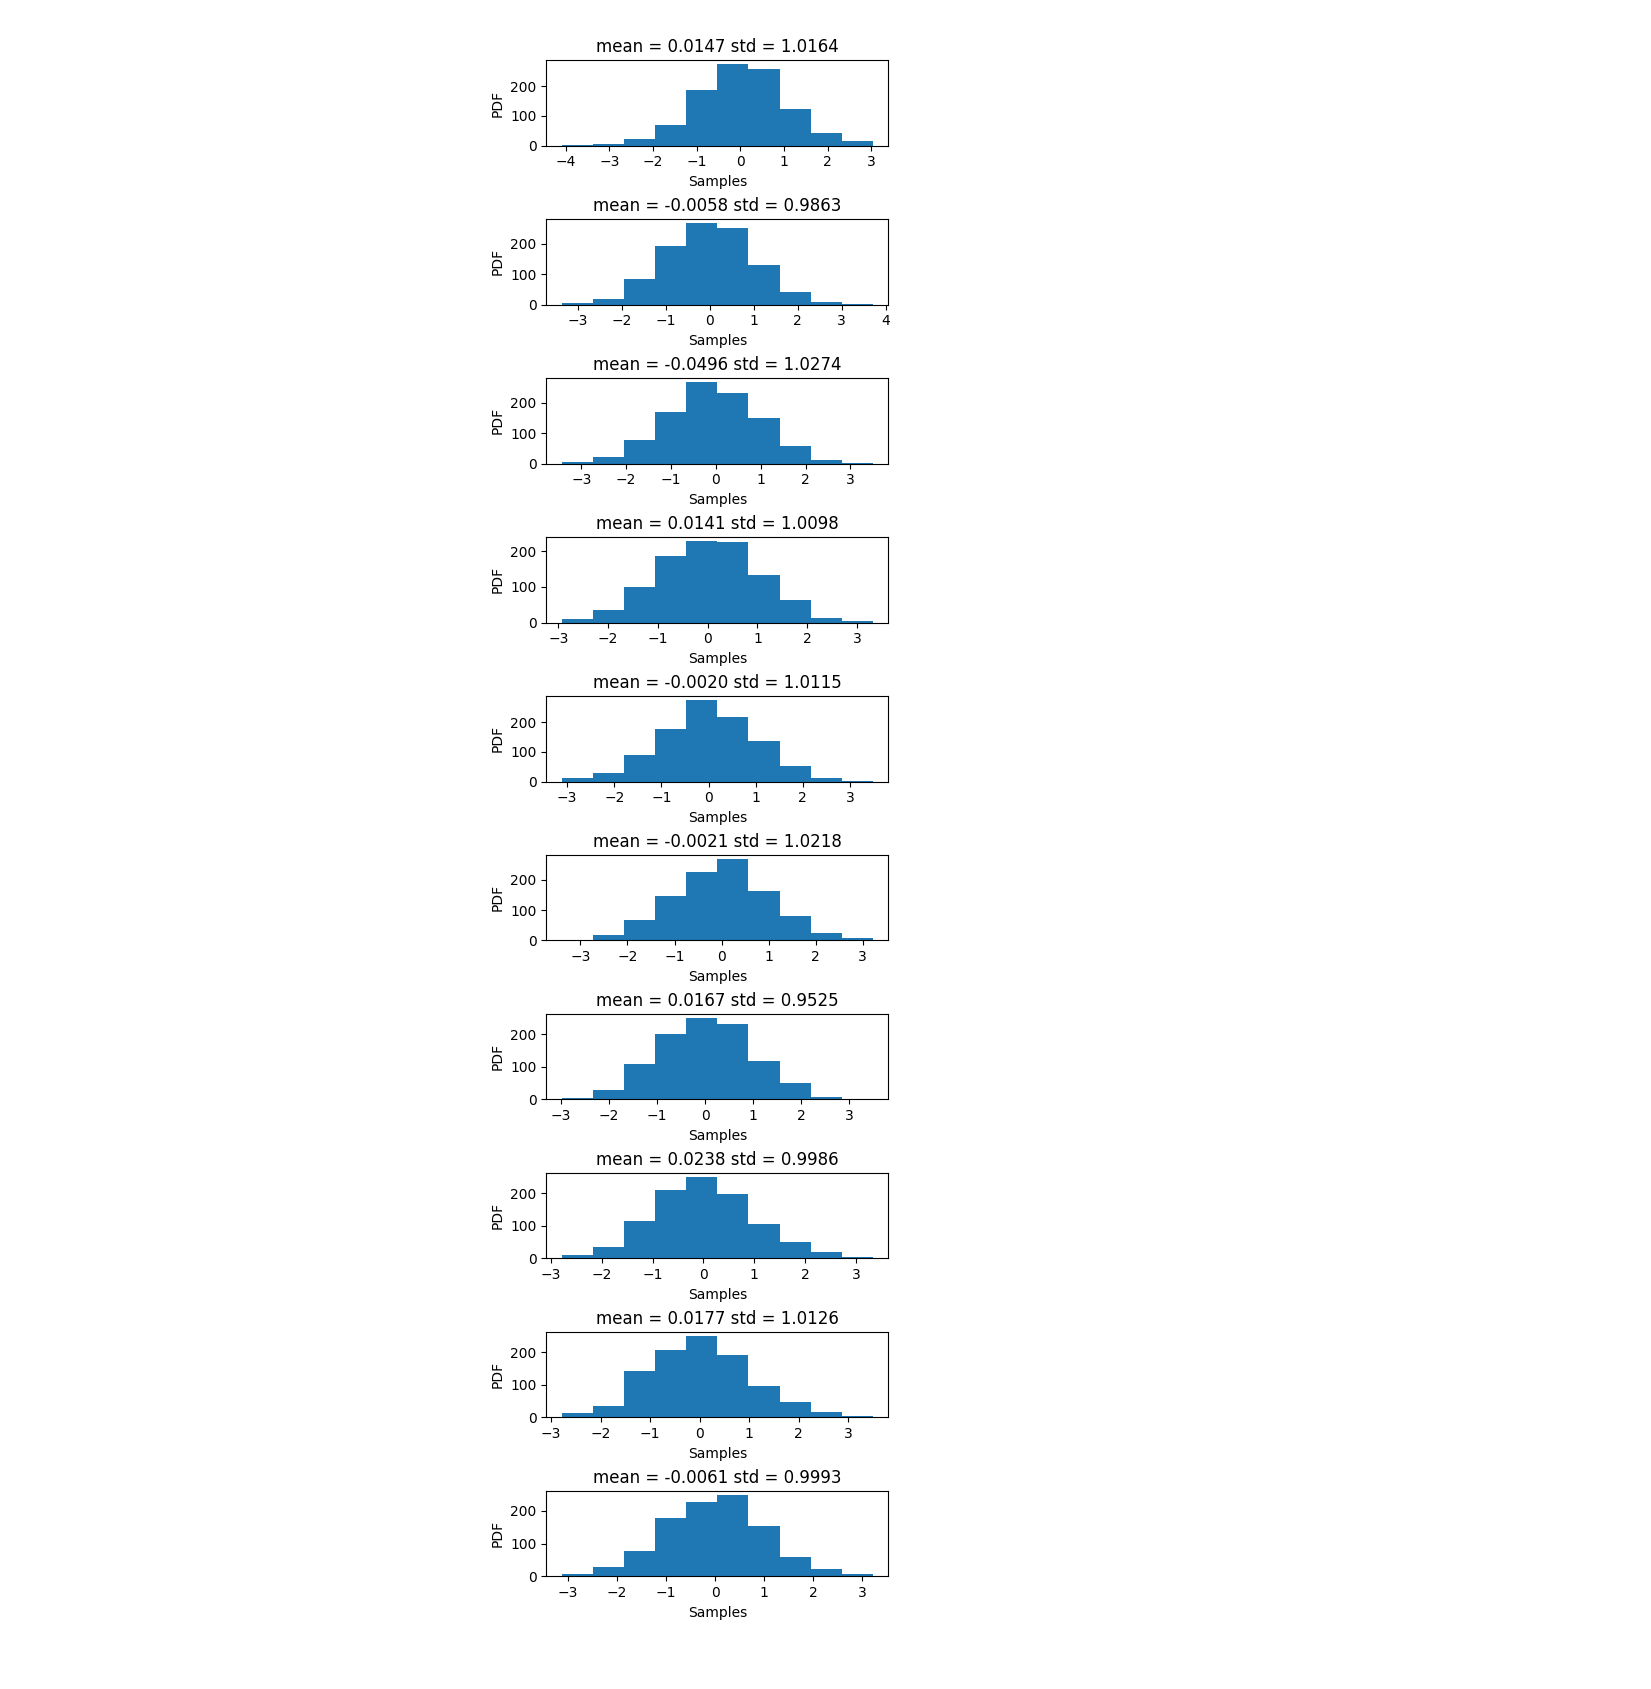
\includegraphics[width=\textwidth]{Graph/b0_nn.png}
		\caption{Program 4: The Bayesian Neural Network weights $b_0$ from top to bottom are the corresponding $i=0$ to $i=9$ histograms for the $10\times1$ vector of $b_0$ (zoom in to see mean and std)}
	\end{center}
\end{figure}
\begin{figure}[h]
	\begin{center}
		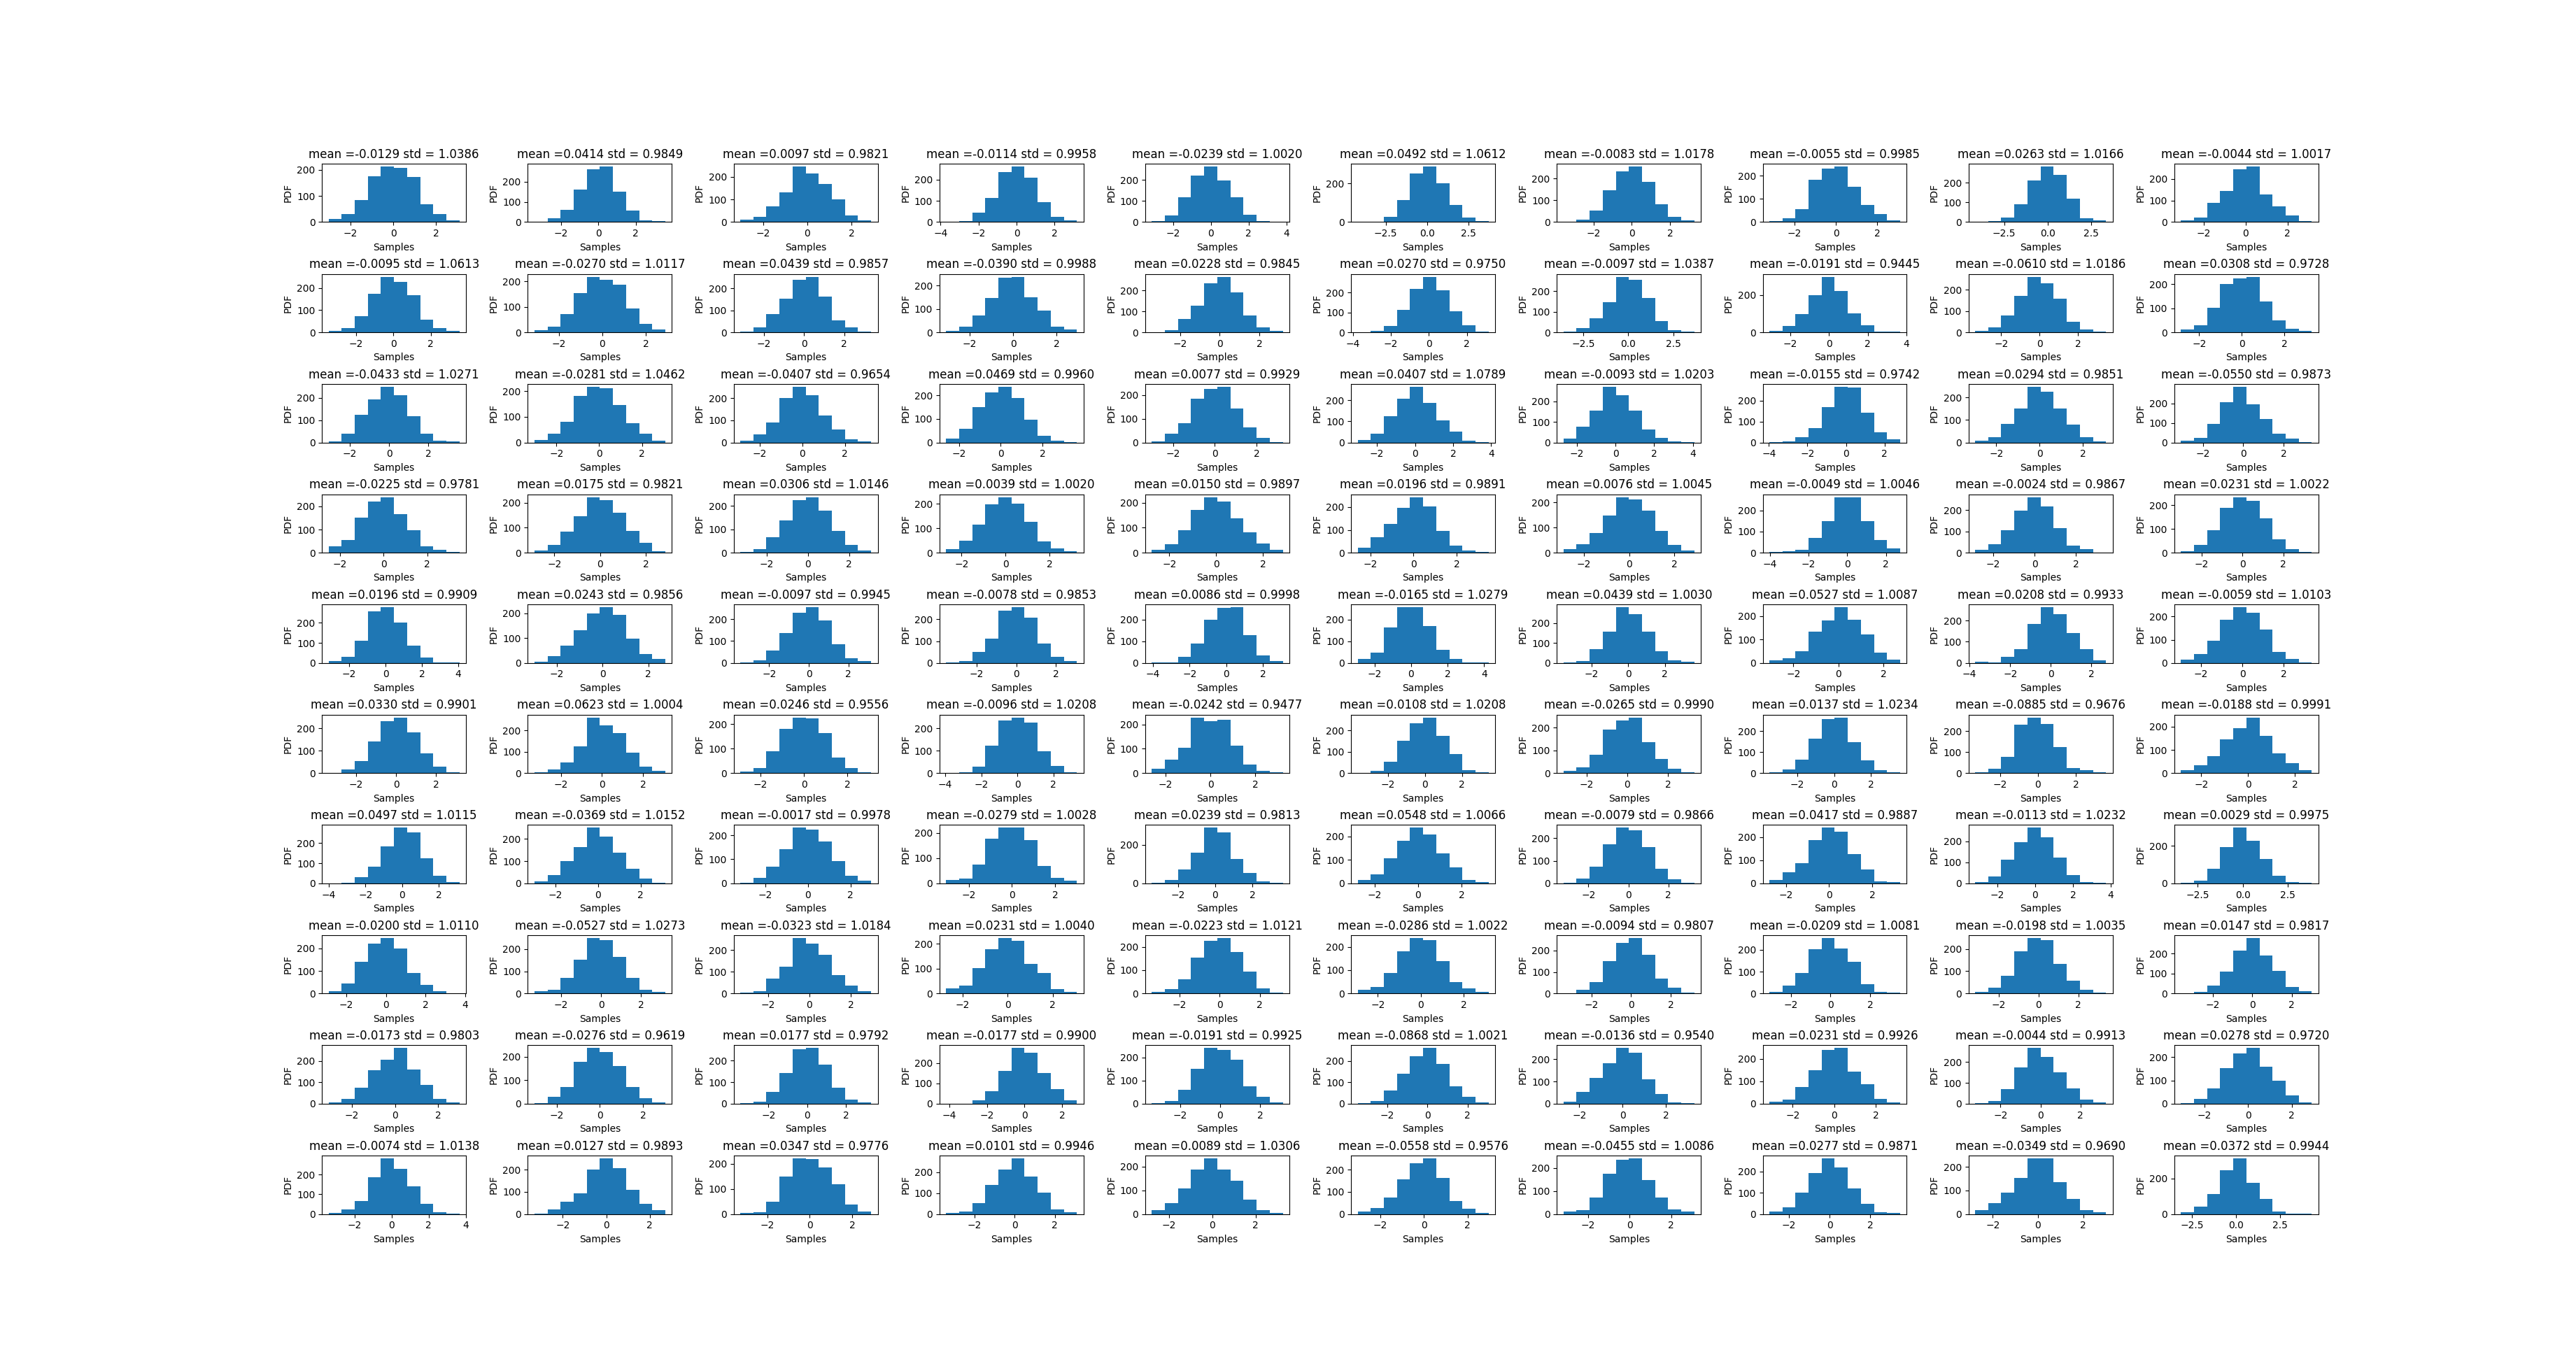
\includegraphics[width=\textwidth]{Graph/W1_nn.png}
		\caption{Program 4: The Bayesian Neural Network weights $W_1$. The histograms are oriented in the same configuration as the $W_1$ matrix i.e histogram $i,j$ corresponds to element $i,j$ of $W_1$ where $W_1$ is a $10\times10$ matrix. Here $i$ corresponds to rows, $j$ to columns.(Zoom in to see the mean and std)}
	\end{center}
\end{figure}
\begin{figure}[h]
	\begin{center}
		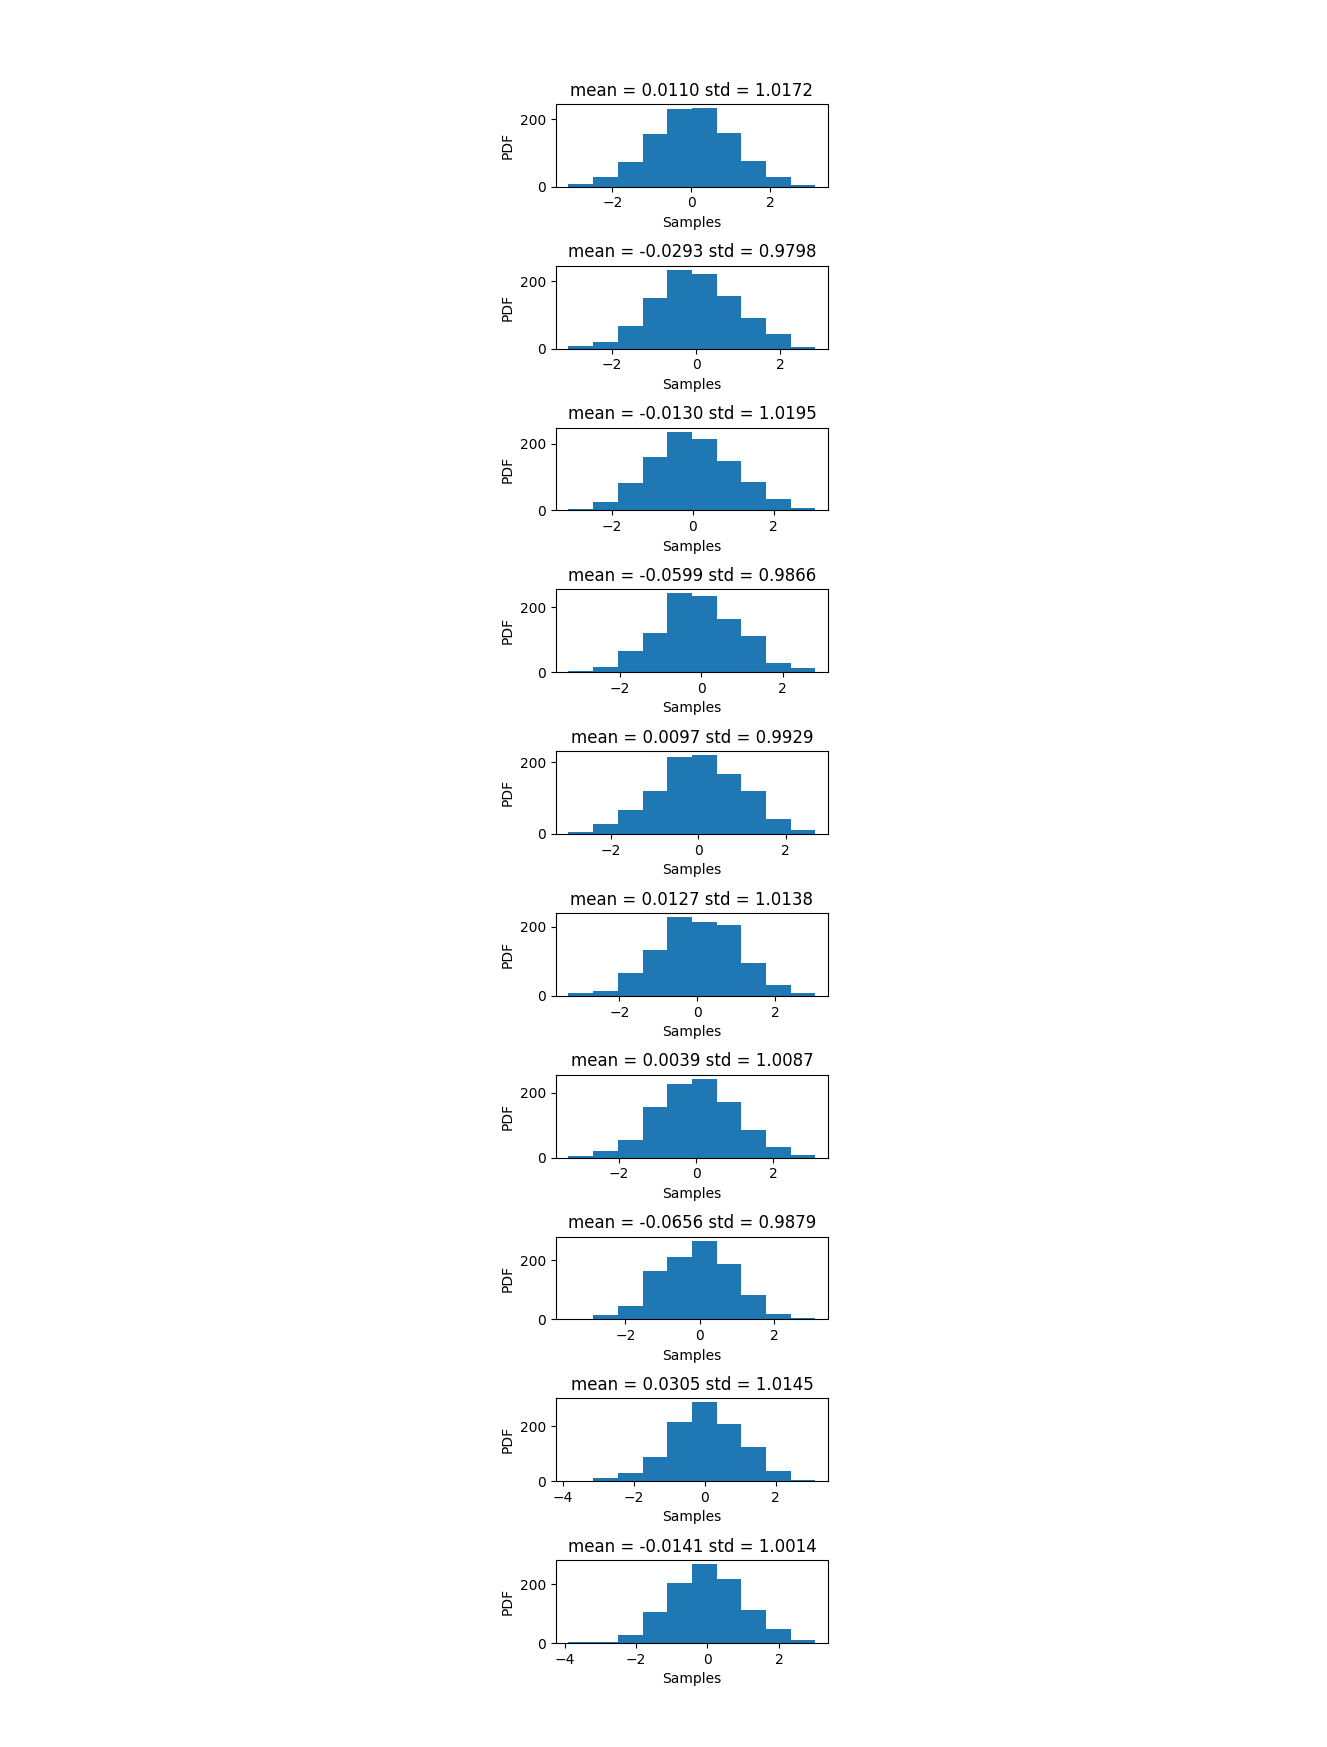
\includegraphics[width=\textwidth]{Graph/b1_nn.png}
		\caption{Program 4: The Bayesian Neural Network weights $b_1$ from top to bottom are the corresponding $i=0$ to $i=9$ histograms for the $10\times1$ vector of $b_1$ (zoom in to see mean and std)}
	\end{center}
\end{figure}
\end{document}
